\documentclass{article}
\usepackage{ctex}
\usepackage{bm}
\usepackage{bbm}
\usepackage{amsmath}
\usepackage{listings}
\usepackage{amsthm}
\usepackage{algorithm,algorithmic}
\usepackage{url}
\usepackage{amssymb}
\usepackage{mathtools}
\usepackage{hyperref}
\usepackage{xcolor}
\newtheorem{theorem}{Theorem}
\newtheorem{example}{Example}
\newtheorem{lemma}{Lemma}
\newtheorem{remark}{Remark}
\def\E{\mathbb{E}}
\def\R{\mathbb{R}}
\DeclareMathOperator{\erf}{erf}
\title{A stochastic convex hull problem}
\begin{document}
\maketitle
\section{General statement}
$p_i$ are points sampled with independent identical distribution in $d$ dimensional space
for $i=1,2,\dots, n, n+1$. We consider the event
$A_n =\{p_{n+1} \in ConvexHull\{p_1,
\dots, p_n\} \}$. $P(A_n)$ is also called
the probability content while $P(A_n^c)
=1-P(A_n)$.
$P(A_n^c)$ increases if $d$ increases,
and it decreases if $d$ increases.

Notice that the event $A^c_n$ is different
from the event that $p_1, \dots, p_{n+1}$
are in convex position.

According to the survey article
\cite{barany2008random},
the problem originally comes from Sylvester's four point problem
in 1864. Then there are two directions afterwards.
One is studying the probability of all points are in convex
position, denoted as $p(n, K)$ in $d$ dimension where $K$ is the convex body
and $n$ is the number of points.
The other direction is to study $P(A_n)$.
The second direction diverges from the first direction
from the paper of Rényi in 1963 \cite{renyi1963konvexe}.

In the paper of Rényi, both the uniform distribution in a bounded region
and the normal distribution is considered.
The setting is constrained in a 2d plane.
When the points follow uniform distribution
in a unit circle, the asymptotic behavior
of the number of vertices is $cn^{1/3}$.
For the standard normal distribution in a plane,
$\E[V_n] \sim 2\sqrt{2\pi \log n}$.

Later on, in the paper of Hervé Raynaud (in the year 1970)
\cite{raynaud1970enveloppe},
the results
of Rényi are extended to higher dimensions.
Both Rényi and Raynaud
based their deductions on integration techniques.
Afterwards, discrete mathematics has been
employed to prove these old results (only the order
is recoverable) \cite{har2011expected}.
\section{Asymptotic result}
In this section, we review two important asymptotic result,
which is obtained in \cite{raynaud1970enveloppe}.
\begin{theorem}
    Let $X_1, \dots, X_n$ be i.i.d. random variables
    drawn from uniform distribution in a $d$-dimensional sphere.
    $H$ is the convex hull of $X_1, \dots, X_n$, which is also
    a random object.
    Then the expected number of vertices of $H$ is
    \begin{equation}
    \E[V_n] \sim f(d)n^{\frac{d-1}{d+1}}
    \end{equation}
    The asymptotic relationship holds when $n\to \infty$.
\end{theorem}
\begin{theorem}\label{thm:x1xnvn}
    Let $X_1, \dots, X_n$ be i.i.d. random variables
    drawn from standard normal distribution in a $d$-dimensional space.
    Then the expected number of vertices of $H$ is
    \begin{equation}
    \E[V_n] \sim g(d) (\log n)^{\frac{1}{2}(d-1)}
    \end{equation}
\end{theorem}
The above two theorems rely on the relationship between
$V_n$ and $F_n$(the $(d-1)$-dimensional faces of $H$).

\begin{equation}\label{eq:fv}
    F_n = (d-1) V_n - d^2 + d + 2
\end{equation}
Using mathematical induction to prove
\eqref{eq:fv}.

% Über die konvexe Hülle von n zufällig gewälhlten Punkten
Below we illustrate the techniques used to prove Theorem
\ref{thm:x1xnvn} by letting $d=2$.
That is, we will show that
\begin{equation}\label{eq:gaussian_2d_evn}
    \E[V_n] \sim 2\sqrt{2\pi \log n}
\end{equation}
starting from
\begin{equation}\label{eq:gaussian_2d_v_n}
    \E[V_n] \sim \frac{n^2}{\sqrt{\pi}}
    \int_{0}^{+\infty} \Phi(p)^{n-2}e^{-p^2}dp
\end{equation}
\eqref{eq:gaussian_2d_v_n} follows
from \eqref{eq:general_2d} with
$\E[|Y_1-Y_2| \Big\vert X_1=X_2=x] = \frac{2}{\sqrt{\pi}}$,
which comes from Lemma \ref{lem:abs_gaussian} with $\sigma=1$.

The first observation is that we can use the approximation
\begin{equation}\label{eq:gaussian_marginal}
    \Phi(p) = 1-\frac{\exp(-p^2/2)}{\sqrt{2\pi} p}
\end{equation}

when $p$ is large.
Given any $\epsilon>0$, the maximal value of $\Phi(p)^{n-2}e^{-p^2}$
is achieved within the interval $[\sqrt{2\log n} - \epsilon, \sqrt{2\log n}]$
for sufficiently large $n$. We can use $\exp(-p^2/2) \sim \frac{1}{n}$
to estimate the boundary.
Therefore:
\begin{equation*}
    \E[V_n] \sim \frac{n^2}{\sqrt{\pi}}
    \int_{\sqrt{2\log n} - \epsilon}^{\sqrt{2\log n}}
    e^{-n\left(\frac{\exp(-p^2/2)}{\sqrt{2\pi}p}\right)-p^2}dp
\end{equation*}
We first make the transformation $u=\sqrt{2\log n} - p$.
\begin{equation}\label{eq:middle}
    \E[V_n] \sim \frac{1}{\sqrt{\pi}}
    \int_{0}^{\epsilon}
    e^{-\left(\frac{\exp(-u^2/2+u\sqrt{2\log n})}{\sqrt{2\pi}(\sqrt{2\log n}-u)}\right)+(2\sqrt{2\log n}u-u^2)}du
\end{equation}
Since $\epsilon $ can be sufficiently small, some terms of $u$
without the coefficient $\sqrt{\log n}$ contribute minor to the integral.
And we can use $u=0$ as an approximation. Therefore,
\eqref{eq:middle} reduces to
\begin{equation*}
    \E[V_n] \sim \frac{1}{\sqrt{\pi}}
    \int_{0}^{\epsilon}
    e^{-\left(\frac{\exp(u\sqrt{2\log n})}{\sqrt{2\pi}(\sqrt{2\log n})}\right)+2\sqrt{2\log n}u}du
\end{equation*}
The next step is to let $t=\sqrt{2\log n} u$, then we have
\begin{equation*}
    \E[V_n] \sim \frac{1}{\sqrt{\pi} \sqrt{2\log n}}
    \int_{0}^{\epsilon \sqrt{2\log n}}
    e^{-\left(\frac{\exp(t)}{2\sqrt{\pi\log n}}\right)+2t}dt
\end{equation*}
Finally, we use $v=\frac{e^t}{2\sqrt{\pi \log n}}$,
then
\begin{equation*}
    \E[V_n] \sim \frac{(2\sqrt{\pi \log n})^2}{\sqrt{\pi} \sqrt{2\log n}}
    \int_{0}^{+\infty}
    e^{-v}vdv = 2\sqrt{2\pi \log n} \approx 5.01 \sqrt{\log n}
\end{equation*}
The above deduction can be extended to handle $d\geq 2$.
\section{Two dimensions}
$(x_i, y_i) \sim p(x,y)$ are i.i.d. distributions
for $i=1,2,\dots, n, n+1$. We consider the event
$A_n =\{(x_{n+1}, y_{n+1}) \in ConvexHull\{(x_1, y_1),
\dots, (x_n, y_n)\} \}$. We give a lower bound on $A_n^c$
(complement) as follows:
\begin{theorem}\label{thm:lower_bound}
    \begin{equation}
        P(A_n^c) \geq \frac{2}{n+1}
    \end{equation}
\end{theorem}
\begin{proof}
We use the method of projection to prove Theorem
\ref{thm:lower_bound}.
Consider a direction $(\cos\theta, \sin \theta)$
characterized by $\theta$. The projection of $(x_i, y_i)$
is given by $x_i \cos\theta + y_i \sin \theta$.
If $\exists \theta$ such that
$x_{n+1}\cos\theta + y_{n+1} \sin \theta$
is larger than $\max_{i=1,\dots, n} \{x_{i}\cos\theta +
y_{i} \sin \theta\}$ or smaller than
$\min_{i=1,\dots, n} \{x_{i}\cos\theta +
y_{i} \sin \theta\}$, $A_n^c$ happens.
Let $z_i = x_i \cos \theta + y_i \sin \theta$,
$z_{\max}=\max\{z_1, \dots, z_n\}$ and
$z_{\min}=\min\{z_1, \dots, z_n\}$.
Then we have $P(A_n^c) \geq P(\exists \theta, z_{n+1} > z_{\max})
+ P(\exists \theta, z_{n+1} < z_{\min})
\geq P(\theta=\theta', z_{n+1} > z_{\max})
+ P(\theta=\theta', z_{n+1} < z_{\min}) $.

Now we compute $P(z_{n+1} > z_{\max})$
for a number $\theta'$.
The PDF of $z=x\cos \theta' + y \sin \theta'$
is given as $p(z)=\int
\frac{p(x, \frac{z-x \cos \theta'}
{\sin \theta'})}{|\sin \theta'|}dx$.
$P(z_{n+1} > z_{\max}) = \int P(z_{\max} < z)p(z)dz
= \int F(z)^n p(z)dz$ where $F(z)$ is the CDF of the
random variable $Z$. Therefore, the integral evaluates
to $\frac{1}{n+1}$. Similarly,
$P(\theta=\theta', z_{n+1} < z_{\min})=
\frac{1}{n+1}$.
\end{proof}

If we consider two directions $\theta_1, \theta_2$
such that $z(\theta_1)=x\cos \theta_1 + y\sin \theta_1$
is independent with $z(\theta_2)=x\cos \theta_2 + y\sin \theta_2$.
For example, If $(X,Y)\sim \mathcal{N}(0, I_2)$,
we choose $\theta_1=0, \theta_2=\frac{\pi}{2}$.
Then
$
P(A_n^c) \geq
P(z_{n+1}(\theta_1)>z_{\max}(\theta_1)
\vee z_{n+1}(\theta_2)>z_{\max}(\theta_2)
\vee z_{n+1}(\theta_1)<z_{\min}(\theta_1)
\vee z_{n+1}(\theta_2)<z_{\min}(\theta_2)
)
$.
Using the inclusion-exclusion principle,
we have
$
P(A_n^c) \geq
4P(z_{n+1}(\theta_1)>z_{\max}(\theta_1))
-4P(z_{n+1}(\theta_1)>z_{\max}(\theta_1)
\wedge z_{n+1}(\theta_2)>z_{\max}(\theta_2)
)
$.
Below we show that
\begin{equation}
    P(z_{n+1}(\theta_1)>z_{\max}(\theta_1)
\wedge z_{n+1}(\theta_2)>z_{\max}(\theta_2))
= \frac{1}{(n+1)^2}
\end{equation}
Let $z=z(\theta_1), z'=z(\theta_2),
z_i = x_i \cos \theta_1 + y_i \sin \theta_1
z'_i = x_i \cos \theta_2 + y_i
\sin \theta_2$,
then
\begin{align*}
    P(z_{n+1}(\theta_1)>z_{\max}(\theta_1)
\wedge z_{n+1}(\theta_2)>z_{\max}(\theta_2))
    &= \iint P(z>z_1 \wedge z'>z'_1)^n p(z,z')dzdz'\\
    &= \iint F(z,z')^n p(z,z')dzdz'\\
    &= \iint F(z)^nF(z')^n p(z)p(z')dzdz'= \frac{1}{(n+1)^2}
\end{align*}
In the last equation, the independence assumption
of $z$ and $z'$ is used.
Therefore, 
\begin{equation}\label{eq:Anc_2_directions}
    P(A_n^c) \geq \frac{4}{n+1} - \frac{4}{(n+1)^2}
\end{equation}



Now we study the case for Gaussian.
Suppose $p(x,y)=\frac{1}{2\pi}\exp(-\frac{x^2}{2}
-\frac{y^2}{2})$,
then the exact formula for $P(A_n^c)$
is (See 1.7 of \cite{kabluchko2020absorption})
\begin{equation}\label{eq:gaussian_2d}
    P(A_n^c) = \frac{n}{\sqrt{\pi}} \int_{-\infty}^{+\infty}
    \Phi^{n-1}(u)e^{-u^2}du
\end{equation}
where $\Phi$ is the CDF of standard normal distribution.
We are interested in the decaying rate of $P(A_n^c)$
when $n\to \infty$, which is given in Lemma \ref{lem:gaussian}
\begin{lemma}\label{lem:gaussian}
If $(X,Y)\sim \mathcal{N}(0, I_2)$, then
\begin{align*}
P(A_n^c )\geq  \sqrt{2}\pi \left(\frac{2}{n+2}
-\frac{1}{n+1}
\right)
\end{align*}
\end{lemma}
\begin{proof}


First use integration by parts:
\begin{align*}
    P(A_n^c) &= \sqrt{2} \int_{-\infty}^{+\infty}
    e^{-u^2/2}d\Phi^n(u)
    =\sqrt{2} \int_{-\infty}^{+\infty}\Phi^n(u)
    ue^{-u^2/2}du \\
    &=2\sqrt{\pi} \int_{-\infty}^{+\infty}
    \Phi(u)^n ud\Phi(u)
\end{align*}
Then use change of variables ($y=\Phi^{n+1}(u)$):
\begin{align*}
    P(A_n^c) 
    =2\sqrt{\pi} \int_{0}^{1}z^n \Phi^{-1}(z)dz
\end{align*}
Using the relationship
$\Phi^{-1}(z)
= \sqrt{2} \erf^{-1}(2z-1)$
where $\erf$ is the error function,
we have
\begin{align*}
    P(A_n^c) 
    =\sqrt{2\pi} \int_{-1}^{1}
    \left(\frac{x+1}{2} \right)^n
    \erf^{-1} (x)dx
\end{align*}
Combining Lemma \ref{lem:bound_erf_integral},
we have $P(A_n^c) \geq  \frac{\sqrt{2}\pi}{n+1}$
approximately, which is a more tight lower bound than
Theorem \ref{thm:lower_bound}.
\end{proof}
\begin{lemma}\label{lem:bound_erf_integral}
    \begin{align}\label{eq:bound_erf_integral}
        \int_{-1}^{1}
    \left(\frac{x+1}{2} \right)^n
    \erf^{-1} (x)dx & \geq \sqrt{\pi}
    \left[\frac{2}{n+2} - \frac{1}{n+1}\right]
    \end{align}
\end{lemma}
\begin{proof}
    When $x>0$, we have the following inequality
    for the inverse error function $\erf^{-1}$
    (See the Maclaurin series of inverse error function
    \cite{inverseErf}).
    \begin{equation}\label{eq:ieq_erf_inverse}
        \erf^{-1}(x) \geq \frac{\sqrt{\pi}}{2}x
    \end{equation}
    In fact, we can replace
    $\erf^{-1}(x)$
    with $\frac{\sqrt{\pi}}{2}x$
    in \eqref{eq:bound_erf_integral} and obtain
    a lower bound.  This is based on the fact
    that $\erf$ is an odd function.
    The deduction is as follows:
    \begin{align*}  
        \int_{-1}^{1}
    \left(\frac{x+1}{2} \right)^n
    \erf^{-1} (x)dx
    &= \int_{-1}^{0}
    \left(\frac{x+1}{2} \right)^n
    \erf^{-1} (x)dx
    +\int_{0}^{1}
    \left(\frac{x+1}{2} \right)^n
    \erf^{-1} (x)dx \\
    &=-\int_{0}^{1}
    \left(\frac{1-x}{2} \right)^n
    \erf^{-1} (x)dx
    +\int_{0}^{1}
    \left(\frac{x+1}{2} \right)^n
    \erf^{-1} (x)dx \\
    &=    
    \int_{0}^{1}
    \left[\left(\frac{x+1}{2} \right)^n-
    \left(\frac{1-x}{2} \right)^n\right]
    \erf^{-1} (x)dx
    \end{align*}
    The term within the square bracket is larger
    than zero, therefore we can use
    the inequality \eqref{eq:ieq_erf_inverse}.

\end{proof}

\subsection{
Special cases for three points in the plane
}
We consider $n=3 (d=2)$.
In this case, $P(A_n)$
is the expected volume of the triangles
whose three vertices are drawn randomly.

\begin{lemma}
    Under the Gaussian assumption of
    Lemma \ref{lem:gaussian},
    we have $P(A_n^c)=\frac{3}{2}
    (1-\frac{\arccos(1/3)}{\pi})
    \approx 0.91$.
\end{lemma}
\begin{proof}
From  \eqref{eq:gaussian_2d},
we should compute the integration
$\int_{\mathbb{R}} \Phi^2(x)e^{-x^2}
dx$.
From \cite{ruben1954moments},
this integral can be computed recursively
by the following formula:
\begin{align}
    \int_{\mathbb{R}} \Phi^n(x)e^{-x^2}
    dx &= \sqrt{\pi} \bar{V}_{n,n}(3) \\
    \bar{V}_{n,n}(x)
    &=\frac{1}{2^n}
    + \frac{n(n-1)}{4\pi}
    \int_{x}^{+\infty}
    \bar{V}_{n-2,n-2}(x'+2)
    \frac{dx'}{x'\sqrt{x'^2-1}}
    \label{eq:recursive}
\end{align}
Notice that \eqref{eq:recursive}
holds for $n\geq 2$. The starting
function is $\bar{V}_{0,0}(x)=1
,\bar{V}_{1,1}(x)=\frac{1}{2}$.
From \eqref{eq:recursive},
we have $\bar{V}_{n,n}(3)=
\frac{1}{4} + \frac{1}{2\pi}
(\frac{\pi}{2} - \arccos\frac{1}{3})
$
Then
\begin{equation}
\int_{\mathbb{R}} \Phi^2(x)e^{-x^2}
dx = \sqrt{\pi}(\frac{1}{2} - \frac{1}{2\pi}\arccos\frac{1}{3})
\end{equation}
Finally,
$P(A_3^c)=\frac{3}{\pi}
\int_{\mathbb{R}} \Phi^2(x)e^{-x^2}
=\frac{3}{2}
(1-\frac{\arccos(1/3)}{\pi})
$.
\end{proof}
If the points are drawn uniformly
from a square $[0,1]^2$, then
$P(A_3^c)=\frac{133}{144}$
(See the formula in \cite{valtr1995probability}
or the result on page 123 in \cite{henze1983random}).

When we require that the distribution is uniform in some bounded region.
An interesting conclusion (from the introduction of \cite{barany2008random})
is that $P(A_3)$ is the largest when
the distribution is uniform in a triangle and
smallest when the distribution is uniform in a disk.

\section{Expected number of vertices}
In section 3 of \cite{efron1965convex},
there is an elegant relationship between
$P(A_n^c)$ and the expected number of vertices
for a convex hull in 2d or 3d dimension.
\begin{equation}\label{eq:vertices}
P(A_n^c) = \frac{1}{n+1}\E[V_{n+1}]
\end{equation}
Using \eqref{eq:vertices}, 
\cite{efron1965convex} gives the formula
of $P(A_n^c)$ in 2d or 3d in Equation (7-5), (7-6).
$P(A_n)$ is also called the probability content.
However, the method used in 
\cite{efron1965convex} is hard to generalize in
higher dimensions.

Using the traditional conclusion on the
asymptotic analysis of $\E[V_n]$
in two-dimensional space,
we can obtain the following
asymptotic behavior for $P(A_n^c)$,
which is consistent with our lower bound
derived above, though the bound is
not tight in the sense of order.


In two dimensions, according to (2.13) of \cite{efron1965convex},
for general spherical distribution,
the expected number of vertices is
\begin{equation}\label{eq:general_2d}
    \E [V_N] = 2\pi \binom{N}{2}
    \int_{\R}\E(|Y_2-Y_1| \Big\vert X_1= x, X_2=x)
    F^{N-2}(x) g^2_2(x)dx
\end{equation}

\eqref{eq:general_2d}
can also be written in a concise form:
\begin{align}
    \E[V_N] & \sim \pi N^2 \int_{\R}F^N(x)G(x)dx 
    \label{eq:E_V_N_F_N_G}\\
    G(x) & = \int_{\R^2} |y_1-y_2| f(x,y_1)f(x,y_2)
    dy_1dy_2
    \label{eq:G_x_y_1_y_2_f}
\end{align}
where $f(x,y)$ is the joint distribution while $F(x)$ is the CDF
of the marginal distribution.

We can show that $G(x)$ is the pdf of a distribution,
that is:
\begin{equation}
    \int_{\R} G(x) dx = 1
\end{equation}

\section{2D uniform distribution}
\begin{theorem}
    $\E[V_n] = O(n^{1/3})$ for uniform distribution
    within a unit circle while
    $\E[V_n] = O(\log(n))$ for uniform distribution
    within a unit square.
\end{theorem}
A refinement for uniform distribution in a 2d circle states that $\E[V_n] \sim C n^{1/3}$ where
the constant $C$ is given as:
\begin{equation}\label{eq:Cn3}
    C = \Gamma\left(\frac{5}{3}\right) \left(\frac{16\pi^2}{3}
    \right)^{1/3} \approx 3.38
\end{equation}
This formula is derived in
Section 3 of \cite{renyi1963konvexe}.

Below we give another derivation of
\eqref{eq:Cn3} starting from (7.13)
of \cite{efron1965convex}, which states that
\begin{equation}\label{eq:uniform_2d_E_v_n}
    \E[V_n] = \frac{2\pi^2}{3}\binom{N}{2}
    \int_{-1}^{1} \Lambda_2^{N-2}(p)\lambda_2^3(p)dp        
\end{equation}
where $\lambda_2(p) = \frac{2}{\pi}\sqrt{1-p^2}$, the marginal
pdf of the uniform distribution over the interior of a unit circle,
and $\Lambda_2(p)$ is the CDF of $\lambda_2(p)$.
\eqref{eq:uniform_2d_E_v_n} can be derived using the property of
uniform distribution, which is summarized in the following lemma:
\begin{lemma}\label{lem:uniform_abs_y_1_y_2}
    Suppose $(X_1, Y_1), (X_2, Y_2)$ follows the uniform distribution
    over the unit circle, and they are independent. Then we have:
    \begin{equation}\label{eq:uniform_23pi_3_lambda_2}
        \E(|Y_2-Y_1| \Big\vert X_1= x, X_2=x)
        = \frac{2}{3}\sqrt{1-x^2}
        =\frac{\pi}{3} \lambda_2(x)
    \end{equation}
\end{lemma}
\begin{proof}
    Let $a=2\sqrt{1-x^2}$. Then the marginal distribution
    of $Y_1|X_1=x, Y_2|X_2=x$ follows the uniform distribution over
    an interval with length $a$.
    Therefore,
    \begin{align*}
        \E(|Y_2-Y_1| \Big\vert X_1= x, X_2=x)
        &= \frac{1}{a^2} \int_0^a \int_0^a |y_1 - y_2| dy_1dy_2 \\
        &= a \int_0^1 \int_0^1 |y_1-y_2|dy_1dy_2 \\
        &=\frac{a}{3}
    \end{align*}
\end{proof}
Using Lemma \ref{lem:uniform_abs_y_1_y_2}, 
from \eqref{eq:general_2d}, we can obtain
\eqref{eq:uniform_23pi_3_lambda_2}.

The first step is to shrink the integration interval.
\begin{align*}
    \int_{-1}^{1} \Lambda_2^{N-2}(p)\lambda_2^3(p)dp
    &=\int_{0}^{1} \left(\Lambda_2^{N-2}(p)
    +(1-\Lambda_2(p))^{N-2}\right)\lambda_2^3(p)dp
\end{align*}
Since $\Lambda_2(p) > \frac{1}{2}$ for $p>0$, the term
$(1-\Lambda_2(p))^{N-2}$ is neglectful when
$N$ is large.
Therefore, we only need to concern about
$\int_{0}^{1} \Lambda_2^{N-2}(p)\lambda_2^3(p)dp$,
Let $p=\cos\theta$, we then have
\begin{align}\label{eq:uniform_integration}
    \int_{0}^{1} \Lambda_2^{N-2}(p)\lambda_2^3(p)dp
    &=\frac{8}{\pi^3}\int_{0}^{\frac{\pi}{2}}
    \left(1+\frac{\sin\theta\cos\theta - \theta}{\pi}\right)^{N-2}
    \sin^4 \theta d\theta
\end{align}
We can change the integral interval to $[0, \epsilon]$
for any constant $\epsilon<\frac{\pi}{2}$ without changing
the asymptotic behavior of the above value.
When $\epsilon$ is small, we can also use the approximation
$\theta \approx \sin\theta$. The term inside
the bracket becomes $1-\frac{1}{2}(2\theta)^3\frac{1}{6}\cdot \frac{1}{\pi}
=1-\frac{2\theta^3}{3\pi}$. We make the change
of variables from $\theta$ to $t$ by:
\begin{align*}
    \frac{t}{N} = \frac{2\theta^3}{3\pi}
\end{align*}
Then $\theta = \left(\frac{3\pi t}{2N}\right)^{1/3}$.
When $N$ is large, we have:
\begin{align*}
\int_{0}^{1} \Lambda_2^{N-2}(p)\lambda_2^3(p)dp
\sim \frac{8}{3\pi^3} \left(\frac{3\pi}{2N}\right)^{5/3}\int_0^{\infty}
\left(1-\frac{t}{N}\right)^{N-2}t^{2/3}dt
\sim\frac{8}{3\pi^3} \left(\frac{3\pi}{2N}\right)^{5/3}
\Gamma\left(\frac{5}{3}\right)
\end{align*}
Then the coefficient $C=\frac{\pi^2}{3}\cdot\frac{8}{3\pi^3} \left(\frac{3\pi}{2}\right)^{5/3}
\Gamma\left(\frac{5}{3}\right)$,
which reduces to \eqref{eq:Cn3}.
\begin{remark}
    We comment on the connection of
    \eqref{eq:uniform_integration} with
    the second last equation on Page 365
    of \cite{affentranger1991convex}.
    Firstly, the case in our consideration is equivalent
    to $s=t=0, d=2$ in \cite{affentranger1991convex}.
    Then the evaluation ($ a=\frac{2^{5/2}}{3\pi}$)
    becomes
    \begin{equation}\label{eq:E_VN_qzero}
        \E[V_N] \sim b_2 N^2 \int_0^1 (1-a \eta^{3/2})^N \eta^{3/2} d\eta         
    \end{equation}

    Notice that the asymptotic behavior of $\E[V_N]$
    only depends on the integral interval $[0, \epsilon]$
    where $\epsilon$ can be arbitrary small.
    We make the transformation $\theta=\sqrt{2\eta}$,
    then we obtain
    $$
    \E[V_N] \sim b_2 N^2 \int_0^1 (1-\frac{2\theta^3}{3\pi})^N
    \theta^4d\theta
    $$
    The integral in the above equation
    is equivalent to \eqref{eq:uniform_integration}.
\end{remark}
\section{Bivariate Cauchy distribution}
Now we consider the case in 2d when the underlining
distribution is Cauchy (spherical symmetric). That is, the pdf is
\begin{equation}\label{eq:pxy_cauchy}
    p(x,y) = \frac{1}{2\pi} \frac{1}{(x^2+y^2+1)^{3/2}}
\end{equation}
The marginal distribution for $X$ is 1d Cauchy,
given by $p(x)=\frac{1}{\pi(1+x^2)}$, which
can be verified by direct integration of
\eqref{eq:pxy_cauchy}.

The 2d Cauchy specified in
\eqref{eq:pxy_cauchy} can be generated in the following way.
Let $y \sim U[0,1]$ and $\theta \sim
U[0, 2\pi]$. Then we obtain $r$
by $r=F^{-1}(y) = \frac{\sqrt{2y-y^2}}{1-y}$.
$F^{-1}$ is the inverse function
of $F(r)=1-(r^2+1)^{-1/2}$, the CDF of
$p(r)= \frac{r}{(r^2+1)^{3/2}}$.
Finally $x,y$ are obtained from polar transformation
of $(r,\theta)$.



From \eqref{eq:general_2d},
we have $g_2(x) = p(x)$ and $F(x)=\frac{1}{2}+ \frac{1}{\pi}\arctan(x)$
for Cauchy distribution.



For the expectation term, we have the following lemma:
\begin{lemma}
    If $(X_1, Y_1), (X_2, Y_2)$ follow the bivariate Cauchy
    distribution, with pdf specified in \eqref{eq:pxy_cauchy}.
    Furthermore, these two random vectors are independent.
    Then we have,
    \begin{equation}\label{eq:cauchy_conditional_expectation}
        \E(|Y_2-Y_1| \Big\vert X_1= x, X_2=x)
        = \frac{\pi}{2}\sqrt{1+x^2}
    \end{equation}
\end{lemma}
\begin{proof}
We list the definite and indefinite integrations
used in the proof first, which come from \cite{integration}.
\begin{align}
    \int_0^{\infty} \frac{dx}{(a^2+x^2)^2}
    & = \frac{\pi}{4a^3} \textrm{ See P108, 47. } \\
    \int \frac{dx}{(x^2+a^2)^{3/2}}
    & = \frac{x}{a^2\sqrt{x^2+a^2}}
    \textrm{ See P27 346.}
    \label{eq:indefinite_inverse_32}\\
    \int \frac{x^2}{(c^2+x^2)^2}dx
    &=-\frac{x}{2(c^2+x^2)}
    +\frac{1}{2c}\arctan\frac{x}{c}
    \textrm{ See P12 137.}
\end{align}
We compute the integration directly:
\begin{align*}
    &\E\left(|Y_2-Y_1| \Big\vert X_1= x, X_2=x\right)
        =\frac{(1+x^2)^2}{4}\iint \frac{|y_1-y_2|}
        {(x^2+y_1^2+1)^{3/2}(x^2+y_2^2+1)^{3/2}}dy_1dy_2\\
        &=\frac{(1+x^2)^2}{2}\int_{\R}\frac{1}{(x^2+y_1^2+1)^{3/2}}
        dy_1\int_{y_1}^{+\infty}\frac{y_2-y_1}
        {(x^2+y_2^2+1)^{3/2}}dy_2 \\
        &=\frac{(1+x^2)^2}{2}\int_{\R}\frac{1}{(x^2+y_1^2+1)^{3/2}}
        \left(\frac{1}{\sqrt{1+x^2+y_1^2}}-y_1\left[\frac{1}{x^2+1}
        -\frac{y_1}{(1+x^2)\sqrt{1+x^2+y_1^2}}\right]\right)dy_1\\
        &=\frac{(1+x^2)^2}{2} \left(\frac{\pi}{2(1+x^2)^{3/2}}
        +\frac{\pi}{2(1+x^2)^{3/2}}\right)\\
        &=\frac{\pi}{2}\sqrt{1+x^2}
\end{align*}
\end{proof}
\begin{lemma}\label{lem:lim_V_N_2d_cauchy}
    For bivariate Cauchy distribution,
$\lim_{N\to \infty}\E(V_N) = \frac{\pi^2}{2} \approx 4.93$.
\end{lemma}
\begin{proof}
From \eqref{eq:general_2d},
we have
\begin{equation}\label{eq:d_2_cauchy_E_V_n}
\E(V_N) = N(N-1)\pi \frac{\pi}{2}\int_{\R}
\sqrt{1+x^2}\frac{1}{\pi^2 (1+x^2)^2}(\frac{1}{2}
+\frac{1}{\pi}\arctan x)^{N-2}dx
\end{equation}
Using the relationship $\arctan x =
\frac{\pi}{2} - \arctan \frac{1}{x}
$, we have (for any given $K>0$):
\begin{align}
    \E(V_N) &\sim \frac{N^2}{2}\int_{K}^{+\infty}
    \frac{1}{(1+x^2)^{3/2}}
    \left(1-\frac{1}{\pi}\arctan \frac{1}{x} \right)^{N}dx\notag \\
    &=\frac{N^2}{2}\int_{0}^{1/K}
    \frac{y}{(1+y^2)^{3/2}}
    \left(1-\frac{1}{\pi}\arctan y\right)^{N}dy
    \label{eq:cauchy_inverse_K_y}\\
\end{align}
When $y$ is small, $\arctan y \approx y$ (Taylor expansion).
Therefore, we can replace $\arctan y$ by $y$ without changing the
asymptotic behavior of the above expression.
Then making another change of variables by
$y=\frac{\pi}{N}t$:
\begin{align*}
    \E(V_N) &\sim \frac{\pi^2}{2}\int_{0}^{N/(K\pi)}
    \frac{tN^3}{(N^2+\pi^2 t^2)^{3/2}}
    \left(1-\frac{t}{N}\right)^{N}dt\\
    &\sim \frac{\pi^2}{2}\int_{0}^{+\infty}
    \frac{tN^3}{(N^2+\pi^2 t^2)^{3/2}}
    e^{-t}dt \sim  \frac{\pi^2}{2}
\end{align*}
\end{proof}
Empirical verification shown in Figure \ref{fig:2d_cauchy}. Use 1000 samples to compute $\E(V_N)$
for each $N$. Notice that as $N$ is large, the expected
number of vertices tend to be a constant (no more than 5).
This behavior is different with Gaussian or unit circle.

\begin{figure}[!ht]
    \centering
    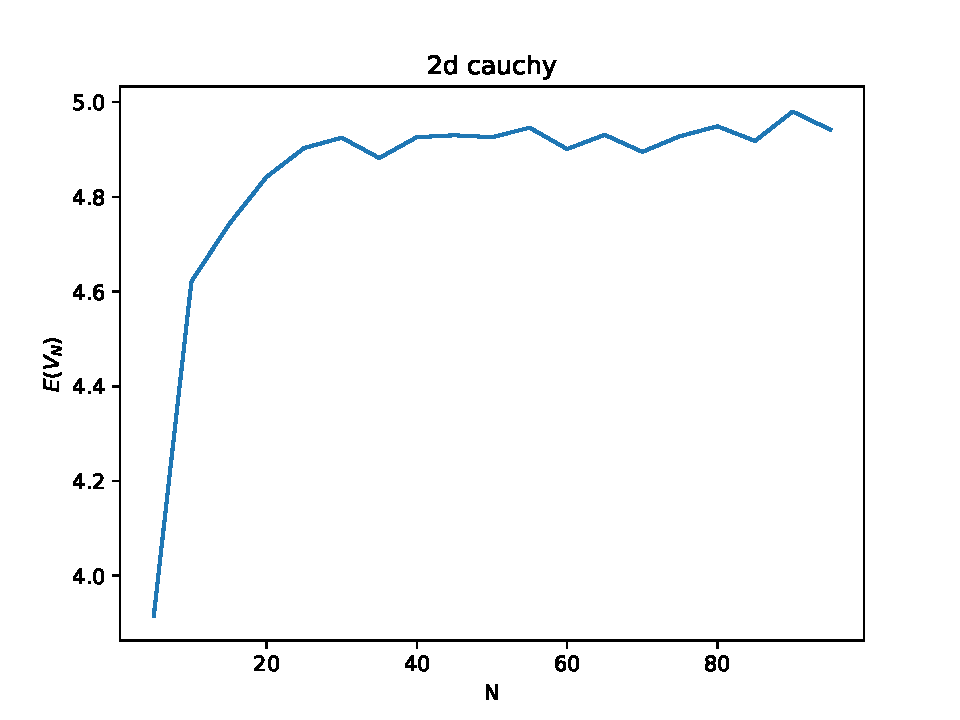
\includegraphics[width=0.6\textwidth]{2d_cauchy_vertices.pdf}
    \caption{}\label{fig:2d_cauchy}
\end{figure}

\section{3d case}
A useful formula is given as Lemma \ref{lem:abs_gaussian}.
\begin{lemma}\label{lem:abs_gaussian}
Suppose $X \in \mathcal{N}(0,1)$,
then $\E[|X|]=\sqrt{\frac{2}{\pi}}$.
Generally, $X \in \mathcal{N}(0,\sigma^2)$,
then $\E[|X|]=\frac{\sqrt{2}\sigma}{\sqrt{\pi}}$.
If $X,Y\sim \mathcal{N}(0,\sigma^2)$ and $X,Y$ are independent,
then $\E[|X-Y|]=\frac{2\sigma}{\sqrt{\pi}}$.
\end{lemma}
A straight line on the plane
can be represented as:
\begin{align}
    x & = p \cos \theta - t \sin \theta \notag \\
    y & = p \sin \theta + t \cos \theta \label{eq:straight_line_rep}
\end{align}
The $p \in \R, \theta \in [0, \pi]$ are fixed while
$t \in \R$ is changeable.
The geometric interpretation of \eqref{eq:straight_line_rep}
is shown in Figure \ref{fig:transformation}.
\begin{figure}[!ht]
    \centering
    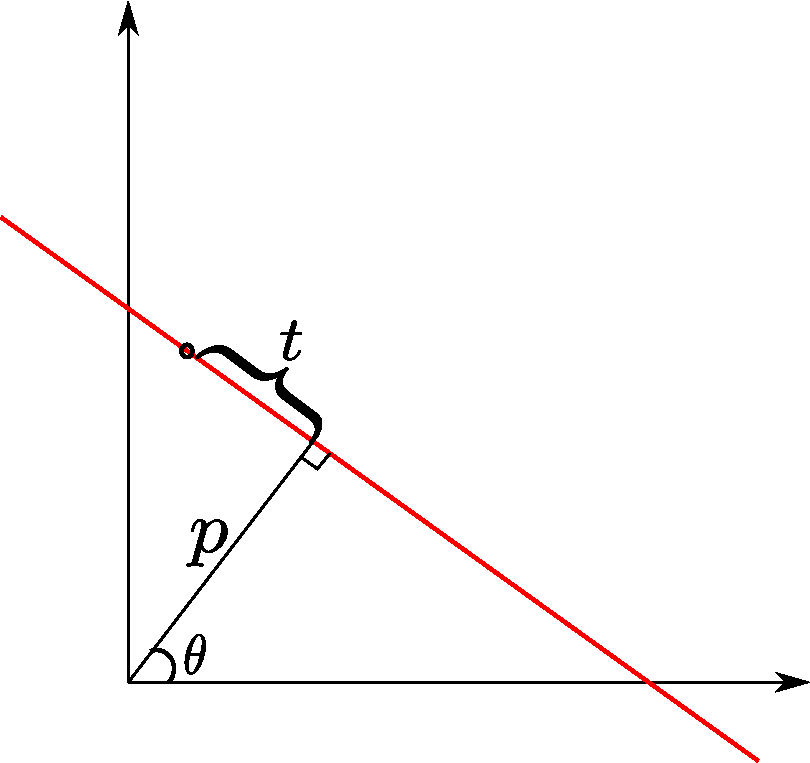
\includegraphics[width=0.6\textwidth]{transformation.pdf}
    \caption{}\label{fig:transformation}
\end{figure}
Below we prove a necessary conclusion for Gaussian distribution.
\begin{lemma}
    The expectation of the area of a triangle
    vertices are drawn independently
    from standard Gaussian distribution is $\frac{\sqrt{3}}{2}$.
\end{lemma}
\begin{proof}
    Let the three points be represented by
    $P_1(x_1, y_1), P_2(x_2, y_2), P_3(x_3, y_3)$.
    We transform the first two points to coordinate
    systems of $(p, \theta, t_1, t_2)$.
    The Jacobian is $|t_1 - t_2|$. Then the first two
    points are represented as
    $P_1(p, \theta, t_1), P_2(p, \theta, t_2)$.
    \begin{equation}\label{eq:EA123_first}
        \E[A_{123}]
        = \frac{1}{2}\int
        |x_3 \cos\theta + y_3 \sin\theta - p|
        (t_2-t_1)^2 f(x_3, y_3) dt_1dt_2 d\theta dp dx_3dy_3
    \end{equation}
    where $f$ is the density function.
    We can use the notation of (2.10) in \cite{efron1965convex}
    and rewrite \eqref{eq:EA123_first} as:
    \begin{equation}\label{eq:EA123_second}
        E[A_{123}] = \frac{1}{2}\int |x_3 \cos\theta + y_3 \sin\theta - p|
        E(L^2_{12} | Q_1=p, Q_2=p)
        \tilde{g}_2(p, \theta)f(x_3,y_3) d\theta dp dx_3dy_3
    \end{equation}
    For spherical-symmetric distribution, from \eqref{eq:EA123_second}
    we can choose the x-axis and obtain
    \begin{equation}\label{eq:EA123_third}
        E[A_{123}] =\frac{\pi}{2}
        \int E(L^2_{12} | X_1=p, X_2=p)
        |x-p|f(x)f^2(p)dxdp
    \end{equation}
    In \eqref{eq:EA123_third},
    the integration of $d\theta dy_3$
    is wiped out,
    it can be made by using the transformation
    $x'_3 = x_3 \cos \theta + y_3 \sin \theta$
    and $y'_3 = x_3 \sin \theta - y_3 \cos \theta$.
    Now we assume standard Gaussian distribution in \eqref{eq:EA123_third}.
    Since $E(L^2_{12} | X_1=p, X_2=p)=2$, we then have (let $p=y/\sqrt{2}$ in the integration)
    \begin{equation}\label{eq:EA123_fourth}
        E[A_{123}] =\frac{\sqrt{\pi}}{2}\int \Big\vert x-\frac{y}{\sqrt{2}} \Big\vert p(x)p(y)dxdy
    \end{equation}
    Since $X-\frac{Y}{\sqrt{2}} \sim \mathcal{N}(0, \frac{3}{2})$,
    from Lemma
    \ref{lem:abs_gaussian},
    we obtain $\E[A_{123}] = \frac{\sqrt{3}}{2}$.
\end{proof}
If the vertices are drawn from uniform distribution
of a unit circle (area equal to $\pi$). Then
$\E[A_{123}] = \frac{35}{48 \pi}$,
which can be computed from (7.13) of 
\cite{efron1965convex} by letting $N=3$.
The result $\E[A_{123}] = \frac{35}{48 \pi}$
can also be computed from \eqref{eq:EA123_third}
by using $E(L_{12}^2|X_1=x,X_2=x)=\frac{\pi^2}{6}f^2(x)
=\frac{2}{3}(1-x^2)$.
This can be seen easily from the fact that
$\E(L^2_{12}) = \frac{2}{3}$ where $X_1, X_2$ are uniform within $[-1,1]$.
Then the integral is scaled to be $[-\sqrt{1-x^2}, \sqrt{1-x^2}]$.
The corresponding integral scales with the coefficient $1-x^2$.
BTW, to compute
$\E(L^2_{12})$ for uniform distributions,
we use the fact that $\E[X_1]=0$ and
$X_1, X_2$ are independent. So that
$\E(L^2_{12}) =\E[(X_1-X_2)^2] 
=\E[X_1^2]+\E[X_2^2]
-2\E[X_1X_2]=2\E[X_1^2]$.

Then the integral equals
\begin{equation}\label{eq:ea123}
    \E[A_{123}] =
    \frac{\pi^3}{12}
    \int_{-1}^{1}\int_{-1}^{1}
    |x-y|f(x)f^4(y)dxdy, \textrm{ where }
    f(x) = \frac{2}{\pi}\sqrt{1-x^2}
\end{equation}
The computation of \eqref{eq:ea123}
can be proceeded as follows:
\begin{align*}
    \E[A_{123}] & =
    \frac{8}{3\pi^2}
    \int_{-1}^{1}\int_{-1}^{1}
    |x-y|\sqrt{1-x^2}
    (1-y^2)^2
    dxdy \\
    & = \frac{8}{3\pi^2}
    \int_{-\frac{\pi}{2}}^{\frac{\pi}{2}}
    \int_{-\frac{\pi}{2}}^{\frac{\pi}{2}}
    |\sin\theta - \sin\varphi|
    \cos^2\theta \cos^5\varphi
    d\theta d\varphi
\end{align*}
where we let $x=\sin \theta, y = \sin \varphi$.
Then we integrate the above expression by parts.
\begin{align*}
    \E[A_{123}] & = \frac{8}{3\pi^2}
    \int_{-\frac{\pi}{2}}^{\frac{\pi}{2}}
    \cos^5\varphi d\varphi
    \int_{-\frac{\pi}{2}}^{\frac{\pi}{2}}
    |\sin\varphi - \sin\theta|
    \cos^2\theta
    d\theta
\end{align*}
Using the indefinite integrals
\begin{align*}
\int \cos^2 \theta d\theta & = \frac{\theta}{2}
+ \frac{\sin 2 \theta}{4} + C\\
\int \sin \theta \cos^2 \theta d\theta & =
- \frac{\cos^3 \theta}{3} + C
\end{align*}
we obtain
\begin{align} \label{eq:abs_integral_computation}
    \int_{-\frac{\pi}{2}}^{\frac{\pi}{2}}
    |\sin\varphi - \sin\theta|
    \cos^2\theta
    d\theta
    &=\left[
    \int_{-\frac{\pi}{2}}^{\varphi}
    (\sin\varphi - \sin\theta)
    \cos^2\theta
    d\theta
    + \int_{\varphi}^{\frac{\pi}{2}}
    (\sin\theta - \sin\varphi)
    \cos^2\theta
    d\theta
    \right]\\
    &=
    \sin\varphi\left(
        \frac{\theta}{2}
    + \frac{\sin 2 \theta}{4}
    \right)
    \Big\vert_{-\frac{\pi}{2}}^{\varphi}
    + \frac{\cos^3\theta}{3}\Big\vert_{-\frac{\pi}{2}}^{\varphi}\notag\\
    &-\frac{\cos^3\theta}{3}\Big\vert_{\varphi}^{\frac{\pi}{2}}
    -\sin\varphi
    \left(
        \frac{\theta}{2}
    + \frac{\sin 2 \theta}{4}
    \right)\Big\vert_{\varphi}^{\frac{\pi}{2}}\notag\\
    &=
    \varphi\sin\varphi
    + \frac{1}{2}\sin\varphi
    \sin 2\varphi
    + 2\frac{\cos^3 \varphi}{3}\notag
\end{align}
Then after simplification, we obtain
\begin{align*}
    \E[A_{123}] =
    \frac{16}{3\pi^2}
    \int_0^{\frac{\pi}{2}}
    (\varphi \sin\varphi \cos^5 \varphi
    + \cos^6 \varphi - \frac{1}{3}
    \cos^8 \varphi
    )d\varphi
\end{align*}
Using symbolic computing package like \texttt{sympy},
finally we obtain $\E[A_{123}]=\frac{35}{48 \pi}$
for uniform distribution within a circle.

For 3d cases, two formulas are essential to compute $\E[V_N]$
for spherical symmetric distribution.
They are listed below:
\begin{align}
    V_N &= \frac{1}{2} F_N + 2 \\
    \E[F_N]&=8\pi \binom{N}{3}
    \int_{\R} 
    E[A_{123}|X_1=X_2=X_3=x] F^{N-3}(x)
    f^3(x) dp\label{eq:gaussian_efn}
\end{align}
For Gaussian distribution, from \eqref{eq:gaussian_efn}
we obtain that $\E[F_N]
= 4\sqrt{3}\pi \binom{N}{3}\int_{\R} \Phi^{N-3}(x)p^3(x)dx$.
The contribution of the order comes from $p^3(x)$.
Using the same method as that used to prove \eqref{eq:gaussian_2d_evn},
we can show that
$\E[F_N] \sim C\log n$.

For the uniform
distribution in the 3d sphere, conditioning on $X_1=X_2=X_3=x$,
$(Y_i, Z_i) (i=1,2,3)$
are uniform distribution in a sphere with
radius $\sqrt{1-x^2}$. Therefore, the expected
area of the triangle is proportional to $1-x^2$.
That is
$\E[A_{123}|X_1=X_2=X_3=x] = \frac{35}{48 \pi}(1-x^2)$.

For uniform distribution
within a sphere,
we get
$\E[F_N]
=\frac{70}{9}
\binom{N}{3}
\int_R F^{N-3}(x)f^4(x)dx$
where $f(x)=\frac{3}{4}(1-x^2)$ is the
marginal pdf.
we can estimate its order by
the following equation:
\begin{align*}
    \int_R F^{N-3}(x)f^4(x)dx
    &\sim (\frac{3}{2})^4
    \int_{1-\epsilon}^{1}
    (1-\frac{3}{4}(1-x)^2)^{N-3}
    (1-x)^4dx \\
    &\sim  (\frac{3}{2})^4
    \int_{0}^{\epsilon}
    (1-\frac{3}{4}y^2)^{N}
    (1-y)^4dy
\end{align*}
Making the change of variable by $\frac{3}{4}y^2=\frac{t}{N}$,
we have
\begin{align*}
    \int_R F^{N-3}(x)f^4(x)dx
    \sim 3\sqrt{3}\Gamma(\frac{5}{2})\frac{1}{N^{5/2}}
\end{align*}
Therefore, we have
\begin{equation}\label{eq:3d_uniform_F_N_value}
    \E[F_N] \sim \frac{35\sqrt{3\pi}}{12}\sqrt{N}     
\end{equation}

The coefficient is approximately 8.95.
This result is consistent with
Theorem 1 of \cite{raynaud1970enveloppe}
when $n=3$.


\section{Cauchy distribution in 3d}
Similar to equation
\ref{eq:EA123_third},
\begin{equation}\label{eq:EA123_third_conditional}
    E[A_{123}|X_1=X_2=X_3=x] =\frac{\pi}{2}
    \int E(L^2_{12} | X_1=x, X_2=x,Y_1=y, Y_2=y)
    |z-y|f_x(z)f_x^2(y)dzdy
\end{equation}
Here $f_x$ is the pdf of $Y|X=x$.
Choosing $d=3$ in \eqref{eq:cauchy_d_dim},
we obtain:
\begin{equation}\label{eq:3d_cauchy_pdf}
    p(x,y,z)=\frac{1}{\pi^2 \left(
        1 + x^2 + y^2 + z^2
    \right)^2}
\end{equation}
Below we first show that
\begin{equation}\label{eq:EL212}
    E(L^2_{12} | X_1=x, X_2=x,Y_1=y, Y_2=y) = 2(1+x^2+y^2)
\end{equation}
\begin{lemma}\label{lemma_xyz_t_distribution}
    If $X, Y, Z$ are multivariate Cauchy distribution whose pdf is
    given in \eqref{eq:3d_cauchy_pdf}.
    Then $\sqrt{\frac{3}{a}} Z|_{X=x,Y=y}$ follows Student's t distribution with $v=3$.
\end{lemma}
\begin{proof}
    The pdf of $Z|_{X=x,Y=y}$
    can be written as
    \begin{align}
        p(z|X=x,Y=y)
        & = \frac{p(x,y,z)}{p(x,y)}\notag \\
        & = \frac{2(x^2+y^2+1)^{3/2}}{
            \pi (1+x^2+y^2+z^2)^2
        } \notag\\
        & = \frac{2}{\pi a^{1/2} (1+\frac{z^2}{a})^2}
        \label{eq:pxy_a}
    \end{align}
    where $ a = 1+x^2+y^2$.
\end{proof}

We can see from \eqref{eq:pxy_a} that
$Z|_{X=x,Y=y}$ is multivariate t distribution with $v=3, p =1, \Sigma=\frac{a}{3}$.
Therefore, $Z|_{X=x,Y=y}/\sqrt{\Sigma}$ follows
t distribution with $v=3$.

\eqref{eq:EL212} is actually computing
$\E[(Z_1 - Z_2)^2]$ with $Z_1, Z_2$ follows distribution with pdf in
\eqref{eq:pxy_a}. Since these two random variables are zero-mean and independent.
We obtain $\E[(Z_1 - Z_2)^2]
=2\E[Z_1^2] = 2 \frac{a}{3} \sigma^2=2a, $
where $\sigma^2$ is the variance of t distribution with $v=3$.
This last deduction follows from 
Lemma \ref{lemma_xyz_t_distribution}.

Below we will show that
\begin{equation}\label{eq:cauchy_a_123}
E[A_{123}|X_1=X_2=X_3=x] = \frac{\pi}{2}(1+x^2)
\end{equation}

We first write the expression for $f_x(z)$
as
$$
f_x(z) = \frac{1+x^2}{2(1+x^2+z^2)^{3/2}}
$$
Then from \eqref{eq:EA123_third_conditional},
we have:
\begin{equation}\label{eq:cauchy_ea123}
    E[A_{123}|X_1=X_2=X_3=x]
    = \frac{\pi}{8} (1+x^2)^3
    \iint_{\R^2} \frac{|z-y|}{(1+x^2+y^2)^2
    (1+x^2+z^2)^{3/2}}dydz
\end{equation}
The computation of 
\eqref{eq:cauchy_ea123} is similar to that of \eqref{eq:ea123}. We need the following two indefinite integration formulas (from \cite{integration}):
\begin{align}
\int \frac{dy}{(a^2+y^2)^2}
& = \frac{1}{2a^3} \left( 
    \frac{ay}{a^2 + y^2} + \arctan \frac{y}{a}
\right)  \textrm{ See P12, 131}  \\
\int \frac{ydy}{(a^2+y^2)^2}
& = -\frac{1}{2(a^2+y^2)}
\textrm{ See P12, 134}
\end{align}
Let $a^2=1+x^2$, we first compute
$\int \frac{|z-y|}{(a^2+y^2)^2}dy$.
The computational process is similar to that of
\eqref{eq:abs_integral_computation},
and we can obtain
\begin{align*}
\int \frac{|z-y|}{(a^2+y^2)^2}dy
&= \frac{1}{a^2 + z^2}
+ \frac{z}{a^3}
\left(
    \frac{az}{a^2+z^2}
    + \arctan \frac{z}{a}
\right)\\
&= \frac{1}{a^2} + \frac{z}{a^3}\arctan\frac{z}{a}
\end{align*}
Then
\begin{align*}
    \iint_{\R^2} \frac{|z-y|}{(1+x^2+y^2)^2
    (1+x^2+z^2)^{3/2}}dydz
    & = \int_{\R} \frac{1}{(a^2+z^2)^{3/2}}\left[\frac{1}{a^2} + \frac{z}{a^3}\arctan\frac{z}{a}\right] dz \\
    &=\frac{2}{a^4}\int_0^{\infty}
    \left(
        \frac{1}{(1+x^2)^{3/2}}
        + \frac{x\arctan x}{(1+x^2)^{3/2}}
    \right)
    dx
\end{align*}
From \eqref{eq:indefinite_inverse_32},
$\int_0^{\infty} \frac{1}{(1+x^2)^{3/2}}dx
= 1
$. On the other hand,
\begin{align*}
    \int_0^{\infty}
    \frac{x\arctan x}{(1+x^2)^{3/2}}dx
    & = \int_0^{\frac{\pi}{2}} y \sin y dy
    \textrm{ where } x = \tan y \\
    & = (\sin y - y \cos y)\Big\vert_0^{\frac{\pi}{2}} = 1
\end{align*}
As a result, we obtain \eqref{eq:cauchy_a_123}.

Now we proceed to compute $\E[F_N]$ for 3d Cauchy.
From \eqref{eq:gaussian_efn},

\begin{align}
\E[F_N]& = \frac{4}{\pi} \binom{N}{3}
\int_{\R} 
\frac{(\frac{1}{2} + \frac{1}{\pi}\arctan x)^{N-3}
}{(1+x^2)^2} dx \label{eq:d_3_cauchy_f_n}\\
& \sim \frac{2}{3\pi} N^3 \int_{K}^{\infty}
\frac{(1-\frac{1}{\pi}\arctan\frac{1}{x})^{N-3}
}{(1+x^2)^2} dx
\end{align}
Similar to the procedure in \eqref{eq:cauchy_inverse_K_y},
we obtain
\begin{equation}
    \lim_{N\to \infty} \E[F_N]
    = \frac{4}{3} \pi^2 \approx 13.159
\end{equation}

Below we conduct experiments to verify our results.


The 3d Cauchy specified in
\eqref{eq:3d_cauchy_pdf} can be generated in the following way.
Let $y \sim U[0,1]$ and $\theta \sim
U[0, \pi], \phi \in U[0, 2\pi]$.
Then we obtain $r$
by $r=F^{-1}(y)$.
$F^{-1}$ is the inverse function
of $F(r)=\frac{4}{\pi}(
-\frac{r}{2(r^2+1)}
+\frac{1}{2}\arctan r
)$, the CDF of
$p(r)= \frac{4}{\pi}\frac{r^2}{(r^2+1)^{2}}$.
We remark here that $1-F(r) \sim \frac{4}{\pi r}$
as $r\to \infty$
using
\begin{align*}
    \arctan r + \arctan \frac{1}{r} & = \frac{\pi}{2} \\
    \arctan \frac{1}{r} & \sim \frac{1}{r} 
\end{align*}

Finally $x,y$ are obtained from polar transformation
of $(r,\theta, \phi)$.
\section{Bivariate t distribution}
Now we consider the case in 2d when the underlining
distribution is Student's t-distribution (spherical symmetric). That is, the pdf is
\begin{equation}\label{eq:pxy_student_t}
    p(x,y) = \frac{1}{2\pi}
    \left(1+\frac{1}{v}(x^2+y^2)
    \right)^{-\frac{v}{2}-1}
\end{equation}
The parameter $v\geq 1$ is the degree of freedom.
Notice that Cauchy distribution is the special
case of t distribution with $v=1$.
The marginal distribution for $X$ is 1d t-distribution, given by
\begin{equation}\label{eq:px_student_t}
    p(x)=
    \frac{\Gamma(\frac{v+1}{2})}
    {\sqrt{v\pi}
    \Gamma(\frac{v}{2})}
    \left(1+\frac{x^2}{v}
    \right)^{-\frac{v+1}{2}}
\end{equation}
which can be verified as follows:
\begin{align*}
\int_{\R} p(x,y) dy & =
\frac{\Gamma(\frac{v}{2} + 1)}
    {\sqrt{v}\pi
    \Gamma(\frac{v}{2})}
    \int_R 
    \left(1+\frac{x^2}{v}+y^2
    \right)^{-\frac{v}{2}-1}dy \\
    & =
    \frac{2\Gamma(\frac{v}{2} + 1)}
        {\sqrt{v}\pi
        \Gamma(\frac{v}{2}) a^{v+1}}
        \int_0^{\frac{\pi}{2}} \cos^v \theta d\theta
\end{align*}
where $a^2=1+\frac{x^2}{v}, y=a\tan \theta$.
Using the formula of Beta function we have
$$
2\int_0^{\frac{\pi}{2}}
\cos^v \theta d\theta
= B\left(\frac{1}{2}, \frac{v+1}{2}\right)
$$
Then after simplification, we can obtain \eqref
{eq:px_student_t}.

Now we extend the result in \eqref{eq:cauchy_conditional_expectation}
to general student's t distribution.
Firstly, from \eqref{eq:pxy_student_t} 
and \eqref{eq:px_student_t},
the conditional distribution can be written as:
\begin{equation*}
    p_{Y|X=x}(y) = \frac{p(x,y)}{p(x)}
    = \frac{\Gamma\left( \frac{v}{2} + 1 \right)}
    {\sqrt{v\pi} \Gamma \left( \frac{v+1}{2} \right)}
    \frac{\left( 1+\frac{x^2}{v} \right)^{(v+1)/2}}
    {\left(1+\frac{1}{v}(x^2+y^2) \right)^{\frac{v}{2}+1}}
\end{equation*}
Let $I(x)=\E(|Y_2-Y_1| \Big\vert X_1= x, X_2=x)$, then
\begin{align*}
   I(x) &= C(x) \iint \frac{|y_2-y_1|
     }{
    \left(1+\frac{1}{v}(x^2+y_1^2) \right)^{\frac{v}{2}+1}
    \left(1+\frac{1}{v}(x^2+y_2^2) \right)^{\frac{v}{2}+1}}
    dy_1dy_2 \\
    & = v^{3/2} C(x)\iint \frac{|y_2-y_1|
    }{
    \left(1+\frac{x^2}{v}+y_1^2 \right)^{\frac{v}{2}+1}
    \left(1+\frac{x^2}{v}+y_2^2 \right)^{\frac{v}{2}+1}
   }
   dy_1dy_2 
\end{align*}
where
\begin{align*}
    C(x) = \frac{\Gamma^2\left( \frac{v}{2} + 1 \right)}
    {v\pi \Gamma^2 \left( \frac{v+1}{2} \right)}
    \left(1+\frac{x^2}{v} \right)^{v+1}
\end{align*}
Let $a^2=1+\frac{x^2}{v}$, we can obtain that
\begin{align*}
    I(x) &= \frac{C(x)v^{3/2}}{a^{2v+1}}
    \int_{-\frac{\pi}{2}}^{\frac{\pi}{2}}
    \int_{-\frac{\pi}{2}}^{\frac{\pi}{2}}
    |\tan \theta - \tan \psi|
    \cos^v\theta \cos^v \psi
    d\theta d\psi \\
    &= C(v)\sqrt{1+\frac{x^2}{v}}
\end{align*}
where $C(v)$ does not contain the term of $x$:
\begin{align*}
    C(v) = \frac{\sqrt{v}\Gamma^2\left( \frac{v}{2} + 1 \right)}
    {\pi \Gamma^2 \left( \frac{v+1}{2} \right)}
    \int_{-\frac{\pi}{2}}^{\frac{\pi}{2}}
    \int_{-\frac{\pi}{2}}^{\frac{\pi}{2}}
    |\tan \theta - \tan \psi|
    \cos^v\theta \cos^v \psi
    d\theta d\psi 
\end{align*}
We can verify that when $v=1$, then $C(v) = \frac{\pi}{2}$,
which coincides with the result of
\eqref{eq:cauchy_conditional_expectation}.

Below we will show that for student's t distribution,
$\lim_{n \to \infty} \E[V_N]$ is a constant value depending on $v$.
We have already computed this constant for $v=1$(Cauchy distribution).
For general $v$, though we are unable to obtain the analytic expression
for the constant, we can at least show that the limit exists and does not depend on $N$.

Let $g(v):=\lim_{n \to \infty} \E[V_N]$. We can even claim the monotonic property
of the function $g(v)$, which is an \textcolor{red}{increasing}
function.

The starting point to prove the existence of $g(v)$ 
is from \eqref{eq:general_2d}.
We also need an expansion of the CDF, which is just the tail area
of the t distribution. Denote the CDF as $F(x)$, then we list the result found in \cite{andrew1976}.
\begin{equation} \label{eq:eq_dv}
    F(x) \sim 1 - D(v)x^{-v} \textrm{ where } D(v)
    =v^{\frac{v}{2}-1} \frac{\Gamma \left(\frac{v+1}{2} \right)}
    {\sqrt{\pi} \Gamma\left(\frac{v}{2}\right)}
\end{equation}
Equation \eqref{eq:general_2d} tells that for bivariate t distribution,
we have
\begin{align}
    \E[V_N] & = 2\pi \binom{N}{2} \int_{\R}
    C(v) \sqrt{1+\frac{x^2}{v}} p^2(x)F^{N-2}(x)dx
    \notag \\
    &\sim \frac{ \mathcal{I}(v)\Gamma^2 \left(\frac{v}{2} +1\right) }
    {\sqrt{v}\pi
    \Gamma^2\left(\frac{v}{2}\right)}  N^2
    \int_{K}^{+\infty} \left(1+\frac{x^2}{v}\right)^{-v-\frac{1}{2}}
    \left(1-D(v)x^{-v} \right)^N dx
    \label{eq:v2bivariate_t_dis}
\end{align}
where
\begin{align}
    \mathcal{I}(v) &= \int_{-\frac{\pi}{2}}^{\frac{\pi}{2}}
    \int_{-\frac{\pi}{2}}^{\frac{\pi}{2}}
    |\tan \theta - \tan \psi|
    \cos^v\theta \cos^v \psi
    d\theta d\psi \notag\\
    &= \frac{4}{v} B\left(v+\frac{1}{2}, \frac{1}{2}
    \right)\label{eq:I_v_analytical}
\end{align}
Making the transformation $\frac{t}{N}=D(v)x^{-v}$
directly, we obtain:
\begin{align}
    \E[V_N] &\sim
    \frac{ \mathcal{I}(v)
    \Gamma^2 \left(\frac{v}{2} +1\right) }
    {\sqrt{v}\pi
    \Gamma^2\left(\frac{v}{2}\right)}  N^2
    \int_{0}^{+\infty} \frac{1}{N^{2+\frac{1}{v}}}\left(\frac{vt^{2/v}}{D^{2/v}(v)}\right)^{v+\frac{1}{2}}
    \left(1- \frac{t}{N} \right)^N \frac{1}{v} t^{-\frac{1}{v}-1} N^{1/v} D^{1/v}(v)dt
    \label{eq:EV_N_general}    \\
    &\sim \frac{ \mathcal{I}(v)
    \Gamma^2 \left(\frac{v}{2} +1\right) }
    {\sqrt{v}\pi
    \Gamma^2\left(\frac{v}{2}\right)} \frac{v^{v-\frac{1}{2}}}
    {D^2(v)} = \frac{\mathcal{I}(v) v \Gamma^2\left(\frac{v}{2}+1\right)}
    {\Gamma^2 \left(\frac{v+1}{2} \right)} 
    =: g(v) \label{eq:E_V_N_v_v_12_D}
\end{align}
That is
\begin{align}
    g(v) &= \frac{\mathcal{I}(v) v \Gamma^2\left(\frac{v}{2}+1\right)}
    {\Gamma^2 \left(\frac{v+1}{2} \right)} \notag \\
    &= \frac{4\sqrt{\pi}
    \Gamma(v+\frac{1}{2})\Gamma^2\left(\frac{v}{2}+1\right)}
    {\Gamma(v+1)\Gamma^2 \left(\frac{v+1}{2} \right)}
    \label{eq:def_g_v}
\end{align}
We can verify that $g(1) = \frac{\pi^2}{2}$,
which is consistent with Lemma \ref{lem:lim_V_N_2d_cauchy}.
Without too much difficulty, we obtain $g(2)=6>g(1)$.
This result is the same with (2.5) in \cite{carnal1970konvexe}
($k$ is the same with $v$).

Though the distribution is not defined at $v=0$,
we can compute formally the value $g(0)=4$.
The number is loosely connected with the lower bound in \eqref{eq:Anc_2_directions}.
But as the independent assumption is violated, this is not
a strict connection.

Using the Stirling's formula for gamma function, we can also
obtain the asymptotic behavior of $g(v)$
as $v$ tends to infinity.
$g(v) \sim 2\pi \sqrt{v}$
as $v\to \infty$.

To verify our above result by experiment,
we need a way
to generate bivariate t distribution.
Let $y \sim U[0,1]$ and $\theta \sim
U[0, 2\pi]$. Then we obtain $r$
by $r=F^{-1}(y) = \sqrt{v}\sqrt{(1-y)^{-2/v}-1}$.
$F^{-1}$ is the inverse function
of $F(r)=
\left(1-(r^2/v+1)^{-v/2}
\right)$, the CDF of
$p(r)= 
\frac{r}{(1+r^2/v)^{v/2 + 1}}$.
Finally $x,y$ are obtained from polar transformation
of $(r,\theta)$.

Before moving to other discussions, we supplement a deduction
of \eqref{eq:I_v_analytical}.
Similar to \eqref{eq:abs_integral_computation},
we first integrate with respect to $\theta$.
\begin{align*}
    \int_{-\frac{\pi}{2}}^{\frac{\pi}{2}}
    |\tan\theta - \tan \psi|
    \cos^v\theta
    d\theta
    &=\left[
    \int_{\psi}^{\frac{\pi}{2}}
    (\tan\theta - \tan\psi)
    \cos^v\theta
    d\theta
    +
    \int_{-\frac{\pi}{2}}^{\psi}
    (\tan\psi - \tan\theta)
    \cos^v\theta
    d\theta
    \right]\\
\end{align*}
To simplify the notation, we define an intermediate function
$F(\psi) = \int_{-\frac{\pi}{2}}^{\psi} \cos^v\theta d\theta$.
Then $ \int_{\psi}^{\frac{\pi}{2}}
\cos^v\theta d\theta
= F(-\frac{\pi}{2}) - F(\psi)$.
Besides, using
$\int_{-\frac{\pi}{2}}^{\frac{\pi}{2}}
\tan\theta \cos^v \theta d\theta= 0
$  (odd function), we obtain that:
\begin{equation*}
    \int_{-\frac{\pi}{2}}^{\frac{\pi}{2}}
    |\tan\theta - \tan \psi|
    \cos^v\theta
    d\theta = 2 \frac{\cos^v \psi}{v}
    +2\tan\psi F(\psi) - \tan \psi F(-\frac{\pi}{2})
\end{equation*}
Notice that the last term disappears in the outer integration.
Then what we are dealing with is:
\begin{equation*}
    \mathcal{I}(v)
    =\int_{-\frac{\pi}{2}}^{\frac{\pi}{2}}
    \cos^v \psi \left[ 2 \frac{\cos^v \psi}{v}
    +2\tan\psi F(\psi) \right] d\psi
\end{equation*}
For the last term in the above equation, we exchange
the sequence of integration order between $\theta$ and $\psi$,
and can obtain immediately:
\begin{align*}
    \int_{-\frac{\pi}{2}}^{\frac{\pi}{2}}
    \cos^v \tan\psi F(\psi) d\psi
    &=  \int_{-\frac{\pi}{2}}^{\frac{\pi}{2}}
    \cos^v \theta d\theta
    \int_{\theta}^{\frac{\pi}{2}}\tan \psi \cos^v \psi d\psi \\
    &=\int_{-\frac{\pi}{2}}^{\frac{\pi}{2}}
    \frac{\cos^{2v}\theta}{\theta}d\theta
\end{align*}
Finally, we obtain:
\begin{equation*}
    \mathcal{I}(v)
    =4\int_{-\frac{\pi}{2}}^{\frac{\pi}{   2}}
    \frac{\cos^{2v}\theta}{\theta}d\theta
\end{equation*}
Using the alternative expression for Beta function,
\eqref{eq:I_v_analytical} is obtained.

\section{N dimensional Cauchy}
The pdf for d dimensional Cauchy is:
\begin{equation}\label{eq:cauchy_d_dim}
    p(\bm{x}) = \frac{\Gamma(\frac{1+d}{2})}
    {\pi^{(d+1)/2} (1+||x||^2)^{(d+1)/2} }
\end{equation}
We can verify that $\int p(x)dx=1$
using high-dimensional spherical integration.
We can also verify that the marginal distribution is Cauchy
distribution in lower dimension.


We follow the ideas in Lemma 2 of \cite{raynaud1970enveloppe},
which discusses the uniform distribution in an n-dimensional sphere,
and we modify it to the n-dimensional Cauchy distribution.
\begin{lemma}\label{lem:p_distribution_d_dim_Cauchy}
    Let $p$ be the distance of a hyperplane generated by $d$ points of $\R^d$ from the origin.
    Now assume these $d$ points are i.i.d. generated from Cauchy distribution with density
    function in \eqref{eq:cauchy_d_dim}.
    The pdf of $p$ is given by
    \begin{equation}\label{eq:p_distribution_d_dim_Cauchy}
        f(p) = k_d (p^2+1)^{-(d+1)/2}
    \end{equation}
    where $k_d$ is the normalization factor given by:
    \begin{equation}\label{eq:k_d_dim_Cauchy}
        k_d = \frac{2 \Gamma \left(\frac{d+1}{2} \right)}{
            \Gamma(\frac{1}{2})
            \Gamma(\frac{d}{2})
        } = \frac{2}{B(\frac{d}{2}, \frac{1}{2})}
    \end{equation}
\end{lemma}
\begin{proof}
    We use the transformation of variables in the integration.
    According to Lemma 1 of  \cite{raynaud1970enveloppe},
    after the integration of angle terms, neglecting the constant coefficient,
    the remaining term in the determinant of the Jacobian matrix becomes
    $|\sum_{i=1}^d (-1)^{d-i} t^{d-1}_1 \dots 
    t^{d-2}_i \dots t^{d-1}_d|$.
    Therefore, we obtain:
    \begin{align}\label{eq:intermediate_f_p_k_d}
        f(p) = k'_d \int_{t_i\geq 0}|\sum_{i=1}^d (-1)^{d-i} t^{d-1}_1 \dots 
        t^{d-2}_i \dots t^{d-1}_d|
        \prod_{i=1}^d \frac{1}{(1+p^2+t_i^2)^{(1+d)/2}}dt_1 \dots dt_d
    \end{align}
    Notice that the term in the denominator
    comes from \eqref{eq:cauchy_d_dim} by using
    the Pythagoras' theorem.
    Let $p_1^2=1+p^2$
    Then we make the change of variables $t_i = p_1d_i$.
    By the scaling effect, we can count the number of $p_1$
    in the two terms of \eqref{eq:intermediate_f_p_k_d}
    respectively. That is, $p_1^{(d-1)d-1}p_1^d / p_1^{(1+d)d}$.
    Then \eqref{eq:p_distribution_d_dim_Cauchy} follows.
    We integrate $f(p)$ directly to obtain the value of $k_d$.
    It reduces to $k_d=\int_0^{\frac{\pi}{2}} \cos\theta^{d-1} d\theta$.
    Finally, \eqref{eq:k_d_dim_Cauchy} follows.
\end{proof}
We can verify Lemma \ref{lem:p_distribution_d_dim_Cauchy}
for $d=2,d=3$ in \eqref{eq:d_2_cauchy_E_V_n} and \eqref{eq:d_3_cauchy_f_n}.
Both the order of $p$ and the coefficient $k_d$ are correct.

Based on
Lemma \ref{lem:p_distribution_d_dim_Cauchy},
we obtain the result
for n dimensional Cauchy.
\begin{theorem}
    Suppose the convex hull is generated by $N$ points in $\R^d$,
    then
\begin{equation}\label{eq:N_infty_F_N_d_Cauchy}
    \lim_{N\to \infty} \E[F_N]
    = \frac{2 \Gamma(\frac{d+1}{2})\pi^{d-\frac{1}{2}}}{d \Gamma(\frac{d}{2})}
\end{equation}
\end{theorem}
\begin{proof}
    The starting integration goes as
    \begin{align}
        \E[F_N]=\binom{N}{d} \int_{\R}
        f(x)(\frac{1}{2} + \frac{1}{\pi}
        \arctan x)^{N-d} dx
    \end{align}
    where $f(x)$ is defined in
    \eqref{eq:p_distribution_d_dim_Cauchy}.
    Then we have (suppose $N-d \to \infty$)
    \begin{align*}
        \E[F_N] \sim & \binom{N}{d} k_d \int
        (x^2+1)^{-(d+1)/2}
        \left(
        1-\frac{1}{\pi} \frac{1}{x}\right)^{N-d} dx \\
        \sim & \binom{N}{d} k_d \frac{\pi^d \Gamma(d)}
        {(N-d)^d}
    \end{align*}
    Or we can use the same techniques as in the deduction for $d=2,3$
    (See \eqref{eq:cauchy_inverse_K_y}), \eqref{eq:N_infty_F_N_d_Cauchy} follows.
\end{proof}
\begin{remark}\label{rem:phase_transition}
    When we assume $N,d$ tend to infinity simultaneously,
    but with a relationship such that $N = \omega(\frac{\pi^d}{\sqrt{d}})$,
    then \eqref{eq:N_infty_F_N_d_Cauchy} holds in a sense that
    the right hand side is the asymptotic order of $\E[F_N]$
    as $d\to \infty$.
    Then using $P(H_{N-1}^c) = \frac{1}{N}\E[V_N] \leq \frac{1}{N}\E[F_N]$
    we can prove that $P(H_{N}^c) \to 0$ for such a relationship of $N$ and $d$.
    But we are more interested in its opposite side. That is:
    when $N,d$ tend to infinity but $N = o(\frac{\pi^d}{\sqrt{d}})$,
    can we obtain $P(H_{N}^c) \to 1$?
\end{remark}
To answer the question put forward in
Remark \ref{rem:phase_transition},
we consider a loose bound for $P(H_N)$:

\begin{equation}
    F_N \leq \binom{V_N}{d} \leq \frac{V^d_N}{d!}
\end{equation}

\begin{equation}
    P(H_N) \leq \E[P_r]
\end{equation}
where $P_r$ is the probability content of a sphere with radius $r$,
and $r= \max\{|X_1|, \dots, |X_N|\}$. Suppose the radius CDF is $1-F(x)$,
then the CDF of $r$ is $(1-F(x))^N$ while $P_x=1-F(x)$.
Then  $\E[P_r] =N\int P_x(1-F(x))^{N-1} |dF(x)|=\frac{N}{N+1}$.
Therefore, $P(H_N^C)\geq \frac{1}{N+1}$.

\subsection{N dimensional t distribution}
Following the same method as in dealing with the N dimensional Cauchy distribution,
we obtain the distribution for $p$, the distance from the origin to the hyperplane as:
\begin{align}
    f(p) & = k_{d,v} \left(1 + \frac{p^2}{v} \right)^{-\frac{vd+1}{2}} \\
    k_{d,v} & = \frac{2}{\sqrt{v} B(\frac{vd}{2},\frac{1}{2})}
\end{align}
Using the expression of $D(v)$ defined in \eqref{eq:eq_dv},
we have:
\begin{align}\notag
    E[F_N] & \sim \binom{N}{d}\int_0^{+\infty} f(p)
    (1-D(v)p^{-v})^{N-d} dp
    = \frac{k_{d,v} v^{(vd+1)/2}\Gamma(d)}{d! v D(v)^d} \\
    & \sim \frac{2 v^{d-1} \pi^{(d-1)/2}
    \Gamma(\frac{v}{2})^{d} \Gamma(\frac{vd+1}{2})}
    {d \cdot \Gamma(\frac{v+1}{2})^d
    \Gamma(\frac{vd}{2})}
    = \frac{2^d \pi^{(d-1)/2}
    \Gamma(\frac{v}{2} +1)^{d} \Gamma(\frac{vd+1}{2})}
    { \Gamma(\frac{v+1}{2})^d
    \Gamma(\frac{vd}{2} + 1)} =:g_d(v)
    \label{eq:F_N_general_d_t}
\end{align}
We can verify that \eqref{eq:F_N_general_d_t} is equivalent with
\eqref{eq:def_g_v} when $d=2$.

In particular, $g_d(0) = \frac{2^d}{(d-1)!}$.
When $d\to \infty$, we have:
$$
g_d(v) \sim \sqrt{\frac{2}{\pi}}\frac{1}{d}\left(
    \frac{\sqrt{\pi}v \Gamma(v/2)}{\Gamma(\frac{v+1}{2})}
\right)^d
$$
Then $P(H_N^c) \leq \frac{1}{N+1}(\frac{1}{d-1} \E[F_{N+1}])$.
When the following condition satisfies, $P(H_N^c) \to 0$:

\begin{equation}
    N = \omega(\frac{1}{d^2} c_v^d) \textrm{ where }
    c_v = \frac{\sqrt{\pi}v \Gamma(v/2)}{\Gamma(\frac{v+1}{2})}
\end{equation}

\subsection{Convex hull in 4d}
Euler's characteristic
(or more generally using Dehn–Sommerville equations
for simplicial polytope):
\begin{equation}
    V_N - E_N + F_N - \tilde{V}_N = 0
\end{equation}   
Using $F_N = 2 \tilde{V}_N$
we can obtain $V_N - E_N + F_N = 0$
\begin{itemize}
    \item $E_N$: the number of edges
    \item $F_N$: the number of faces (triangles)
    \item $\tilde{V}_N$: the number of volumes (tetrahedra)
\end{itemize}
We can use the generalized lower bound theorem
(See Theorem 1.1 in \cite{juhnke2018balanced} for detail) to obtain the
inequality relationship between $V_N$ and $F_N$: $F_N \geq 3V_N - 10$.

In higher dimensions, we have:
\begin{equation}\label{eq:F_V_upper}
    F_N \geq (d-1) V_N - (d+1)(d-2)
\end{equation}

Equation \eqref{eq:F_V_upper} comes from
Corollary 19.6 of \cite{brondsted2012introduction}.

Another inequality comes as:
\begin{align}
    F_N & \leq \Phi_0(d, V_N) \\
    \Phi_0(d,p) & = \binom{p-m-1}{n}
    + \binom{p-n-1}{m}
\end{align}
where $m=\lfloor \frac{d-1}{2} \rfloor$
and $n=\lfloor \frac{d}{2} \rfloor$.
See Corollary 18.3 in \cite{brondsted2012introduction}.

\section{Random notes}
Expected volume and probability content are two different concepts.
Only in the case of uniform distribution within a sphere are they equivalent
by a scaling factor of the volume of the hyper-ball.

In \cite{affentranger1991convex},
the expected volume for different distribution in $\R^d$ is discussed in detail.

In \cite{eddy1981convex}, three cases are
categorized for the convex hull with spherically symmetric
distribution: algebraic tail, exponential tail and truncated tail.
I think this conceptual construction is
loosely connected with three typical distributions:
t-distribution, Gaussian and uniform distribution in a sphere.

\section{Exponential Tails}
Exponential tails: $\Pr(R>r) = C(\alpha, \beta, \gamma) r^{\alpha} \exp(-\gamma r^{2\beta})$.
When $\alpha=0, \beta=2, \gamma=\frac{1}{2}$,
this distribution is standard multivariate distribution in polar coordinate of $\R^d$.

Below we first consider a simple case in $\R^2$,
$\alpha=2,\beta=1, \gamma=\frac{1}{2}$.
The pdf of the distribution in Cartesian coordinate
can be written
as 
\begin{equation}\label{eq:exponential_tail_2d_alpha_2}
    p(x,y) = C(x^2+y^2) \exp(-\frac{x^2+y^2}{2})    
\end{equation}
.

Based on \eqref{eq:general_2d}, we would like to obtain $\E[V_N]$.
In the case $\alpha=0$, $\E(|Y_2-Y_1|X_1=x,X_2=x)$ is a constant.
But we will show that in the case of $\alpha=2$,
$\E(|Y_2-Y_1|X_1=x,X_2=x)$ is asymptotically a constant as $|x|\to\infty$.
Notice that in the derivation of \eqref{eq:gaussian_2d_v_n},
only the asymptotic expression of each element is required.
Therefore we conclude that
$\lim_{N\to \infty} \E[V_N]$ is also of the order $\sqrt{\log n}$
but the coefficient is different.
\begin{lemma}\label{lem:limit_expectation_y1_minus_y2}
If $(X_1,Y_1), (X_2,Y_2)$ are independently
sampled from the distribution specified in \eqref{eq:exponential_tail_2d_alpha_2}.
Then 
\begin{equation}\label{eq:abs_y1_y2_x_exp_tail}
\lim_{x\to \infty} \E[|Y_1-Y_2| \Big\vert X_1=X_2=x] = \frac{2}{\sqrt{\pi}}
\end{equation}
\end{lemma}
Notice that in \eqref{eq:abs_y1_y2_x_exp_tail}, the asymptotic constant is the same
with the case when $\alpha=0$. Then we conclude that the asymptotic behavior
of $\E[V_N]$ is exactly the same for $\alpha=0$ and $\alpha=2$.
\begin{proof}
    The marginal distribution $p(x)=\sqrt{2\pi} C(1+x^2) \exp(-x^2/2)$.
    Then the conditional distribution is $p(y|x)
    = \frac{(x^2+y^2)\exp(-y^2/2)}{(1+x^2)\sqrt{2\pi}}$.
    \begin{align*}
        \E(|Y_2-Y_1|X_1=x,X_2=x)
        & = \iint |y_2-y_1| p(y_1 |x_1=x)p(y_2 | x_2=x)
        dy_1dy_2 \\
        & = \frac{1}{2\pi(1+x^2)^2} \iint |y_1-y_2|
        (x^2+y_1^2)(x^2+y_2^2) \exp(-\frac{1}{2} (y^2_1+y^2_2)) dy_1dy_2\\
        &= \frac{C_1 x^4 + C_2x^2+C_3}{(1+x^2)^2}
    \end{align*}
    We see that the limit is $C_1$ as $x\to \infty$ where
    \begin{align*}
        C_1 &= \frac{1}{2\pi} \iint |y_1-y_2| \exp(-\frac{1}{2} (y^2_1+y^2_2)) dy_1dy_2 \\
        &= \frac{1}{2\pi} \iint |\sin \theta- \cos \theta|
        r^2\exp(-r^2/2) drd\theta \\
        &= \frac{2}{\sqrt{\pi}}
    \end{align*}
\end{proof}

We can generalize the above result to any $\alpha>0$.
\begin{lemma}
    If $(X_1,Y_1), (X_2,Y_2)$ are independently
    sampled from the distribution specified as
    \begin{equation}\label{eq:exponential_tail_2d_alpha}
        p(x,y) = C(x^2+y^2)^{\alpha/2} \exp(-\frac{x^2+y^2}{2})    
    \end{equation}   
    Then 
    \begin{equation}\label{eq:abs_y1_y2_x_exp_tail_2}
    \lim_{x\to \infty} \E[|Y_1-Y_2| \Big\vert X_1=X_2=x] = \frac{2}{\sqrt{\pi}}
    \end{equation}
    \end{lemma}
The key idea to prove the above lemma is using the fact that
$(x^2+y^2)^{\alpha/2} \sim x^{\alpha}$ as $x\to \infty$.
Other computation is just the same as the proof of Lemma \ref{lem:limit_expectation_y1_minus_y2}.

Next we discuss the influence of the coefficient $\gamma$, which also does not influence $\E[V_N]$.
This is because we can make some transformations to normalize $\gamma=\frac{1}{2}$.
See also the discussion in Section 6 of \cite{efron1965convex}, which states that
linear transformation (scaling and translation)
does not influence the expected number of vertices.

Below, we give the simulation scheme
for $p(x,y)=C\exp(-(x^2+y^2)^\beta)$.
In polar coordinate, it can be written as
$p(r) = C r \exp(-r^{2\beta})$.
Its CDF is given by $F(r) = \frac{1}{\Gamma(1/\beta)}
\gamma(\frac{1}{\beta}, r^{2\beta})$,
or in the regularized lower gamma function
form $F(r) = P(\frac{1}{\beta}, r^{2\beta})$.
We can use numerical routine to obtain $F^{-1}(u)$
for $u\in (0,1)$. Thus we get the random generator for
the radius direction.

If we consider the case $\alpha=0$ while $\beta > 0$,
that is
\begin{equation}\label{eq:joint_pdf_beta_x_y}
    p(x,y)=\frac{\beta}{\pi 2^{1/\beta} \Gamma(1/\beta)}
    \exp \left(-\frac{(x^2+y^2)^{\beta}}{2} \right)        
\end{equation}

We make an approximation of $p(x,y)$ when $y$ is fixed and $x\to \infty$.
That is
$p(x,y)=C \exp(-x^{2\beta}/2) \exp(-\beta y^2 x^{2\beta-2}/2)$.
In such a case $Y|X=x$ is a Gaussian.
%We get the marginal distribution easily as 
%$$
%p(x) =C x^{1-\beta} \exp(-x^{2\beta}/2)
%$$
Besides, from \eqref{eq:G_x_y_1_y_2_f},
$$
G(x) = \int_{\R^2}
|y_1 - y_2| p(x,y_1)p(x,y_2)dy_1dy_2
\sim C_{\beta} x^{3-3\beta} \exp(-x^{2\beta})
$$
where
$$
C_{\beta}
= \frac{\beta^{1/2}}{\pi^{3/2} 2^{\frac{2}{\beta}-2}
\Gamma^2(\frac{1}{\beta})}
$$
For the CDF of the marginal distribution,
we have the following lemma:
\begin{lemma}\label{lem:phi_asymptotic}
    Suppose the joint pdf of $(X,Y)$
    is given in \eqref{eq:joint_pdf_beta_x_y}, then
    the marginal CDF $F(x)$ satisfies
$$
1-F(x) \sim C\frac{\exp(-x^{2\beta}/2)}{x^{3\beta - 2}}
$$ as $x\to \infty$,
where
$$
C=\frac{1}{2^{1/\beta} \Gamma(1/\beta)} \sqrt{\frac{2}{\beta \pi}
}$$
\end{lemma}
\begin{proof}
    We can write down the integration
    of $1-F(x)$
    explicitly as:
    \begin{align}
    1-F(x)  & = \frac{\beta}{\pi 2^{1/\beta} \Gamma(1/\beta)}
    \int_x^{+\infty}   \int_{\R} \exp \left(
        -\frac{(u^2+y^2)^{\beta}}{2}\right)
        dudy \notag \\
        & \sim \frac{\beta}{\pi 2^{1/\beta} \Gamma(1/\beta)}
        \int_x^{+\infty}  \exp(-\frac{u^{2\beta}}{2})
        \int_{\R} \exp \left(
            -\frac{\beta u^{2\beta - 2} y^2 }
            {2}
            \right)
            dudy\notag \\
        & = \frac{\beta}{\pi 2^{1/\beta} \Gamma(1/\beta)}
        \int_x^{+\infty} \frac{1}{u^{\beta-1}}
        \exp
        \left(
            -\frac{u^{2\beta}}{2}
        \right)du
        \int_{\R} \exp \left(
            -\frac{\beta v^2}{2}\right)
            dy \notag\\
        & = \frac{\beta}{\pi 2^{1/\beta} \Gamma(1/\beta)}
        \cdot \sqrt{\frac{2\pi}{\beta}}
        \int_x^{+\infty} \frac{1}{u^{\beta-1}}
        \exp
        \left(
            -\frac{u^{2\beta}}{2}
        \right)du
        \label{eq:integration_by_parts} \\
        &
        = \frac{\beta}{ 2^{1/\beta} \Gamma(1/\beta)}
        \cdot \sqrt{\frac{2}{\beta \pi}}
        \left(\frac{1}{\beta}
        \frac{\exp(-x^{2\beta}/2)}{x^{3\beta -2}}
        -(3\beta-2)
        \int_x^{+\infty} \frac{1}{u^{3\beta-1}}
        \exp
        \left( 
            -\frac{u^{2\beta}}{2}
        \right)du \right)\notag
    \end{align}
    In \eqref{eq:integration_by_parts},
    we proceed by integration by parts.

\end{proof}
\textcolor{red}{We conclude that
$\lim_{N\to \infty} \E[V_N]$
is of the order $ 2\sqrt{2\pi \beta} \sqrt{\log n}
$ for general $\beta>0$.}
To prove this, we use the same procedure for $\beta=1$
in \eqref{eq:gaussian_2d_v_n}.
From \eqref{eq:E_V_N_F_N_G},
$$
E[V_N] = \pi N^2\int_{\R}G(x)F^N(x)
dx\sim \pi C_\beta
N^2 \int_{\R}
x^{3-3\beta} \exp(-x^{2\beta}) \left(
1-C\frac{\exp(-x^{2\beta}/2)}{x^{3\beta-2}}
\right)^N dx
$$
We deal with 
\begin{align*}
    N^2 \int_{(2\log n)^{1/(2\beta)}-\epsilon}^{(2\log n)^{1/(2\beta)}}
    x^{3-3\beta}\exp\left(
    -x^{2\beta} -N
    C\frac{\exp(-x^{2\beta}/2)}{x^{3\beta-2}}
 \right) dx
\end{align*}
The term $x^{3-3\beta}$ takes the value
$(2\log N)^{\frac{3-3\beta}{2\beta}}$ directly.

Let $x=(2\log N)^{1/(2\beta)}-u$ (change of variables).
Only reserving dominant terms in $\log N$:
$
x^{2\beta} = 2\log N - 
2\beta
(2 \log N)^{1-1/(2\beta)}u$.

\begin{align*}
    (2\log N)^{\frac{3-3\beta}{2\beta}}
    \int_{0}^{\epsilon}
\exp\left(
    2\beta (2\log N)^{1-\frac{1}{2\beta}} u -
    C\frac{\exp(\beta (2\log N)^{1-\frac{1}{2\beta}} u)}{(2\log N)^{\frac{3\beta-2}{2\beta}}}
 \right) du
\end{align*}
Let $t=\beta (2\log n)^{1-\frac{1}{2\beta}}u$
\begin{align*}
    \frac{(2\log N)^{\frac{3-3\beta}{2\beta}}
    }{\beta(2\log N)^{1-\frac{1}{2\beta}}}
    \int_{0}^{\epsilon}
\exp\left(
    2t -
    C\frac{e^t}{(2\log N)^{\frac{3\beta-2}{2\beta}}}
 \right) dt
\end{align*}
Then let $v=C\frac{e^t}{(2\log N)^{\frac{3 \beta - 2}{2\beta}}}$
\begin{align*}
   \frac{1}{C^2\beta} (2\log N)^{\frac{2}{\beta} - \frac{5}{2}}
    (2\log N)^{\frac{3 \beta - 2}{\beta}}
    \int_{0}^{+\infty}
ve^{-v}dv
%\stackrel{\cdot}{=}
= \frac{\sqrt{2}}{C^2\beta}
\sqrt{\log N}
\end{align*}
Finally, we obtain $\E[V_N] 
\sim \pi C_{\beta} \cdot \frac{\sqrt{2}}{C^2\beta} \sqrt{\log N}
 = 2\sqrt{2\pi \beta} \sqrt{\log N}$.

Notice that the coefficient increases with $\beta$,
which is consistent with the fact that the number of nodes increase
more rapidly 
when the distribution decreases faster.

\section{Linear combination of algebraic tails}
When we consider the distribution in the linear combination
of pdf with different $v_i$.
Then the dominant term is the one with minimal $v_i$,
which is summarized in the following theorem.

\begin{theorem}\label{thm:combination_all}
Suppose the pdf is the finite linear combination of t-distribution with
different degrees of freedom, defined as:
\begin{equation}
    p(x,y) = \sum_{i=1}^k C_i (1+\frac{1}{v_i}(x^2+y^2))^{-v_i/2 - 1}
\end{equation}
Then the asymptotic rate of the number of vertices $\E[V_N]$
depends only the dominant term:
\begin{equation}
    \E[V_N] \sim g(\min_{1\leq i\leq k} v_i)
\end{equation}
where $g(v)$ is defined in \eqref{eq:def_g_v}.
\end{theorem}
Theorem \ref{thm:combination_all} tells us that
the rate $\E[V_N]$ is not an average from $v_1, \dots, v_k$
weighted by $C_1, \dots, C_k$. Instead, it is totally determined by
the smallest $v_i$.

\begin{proof}
    WLOG, we suppose $v_1 < v_2 < \dots < v_k$.
    We can rewrite \eqref{eq:general_2d}
    in the following form of
    \begin{align}
        \Lambda(x) &= \int_{\R} |y_1-y_2| f(x, y_1) f(x,y_2)
        dy_1dy_2
        \\
        \E[V_N]
        &\sim \pi N^2 \int_{\R} F^{N}(x) \Lambda(x)dx
    \end{align}
    First we compute $\Lambda(x)$,
    we only reserve the dominant term about $x$.
    Let $v=v_1$ to simplify the notation.
    We then have
    \begin{equation}
        \Lambda(x) \sim \frac{ \mathcal{I}(v)\Gamma^2 \left(\frac{v}{2} +1\right) }
        {\sqrt{v}\pi^2
        \Gamma^2\left(\frac{v}{2}\right)} (1+x^2/v)^{-v-\frac{1}{2}} C^2_1
         \left( \frac{\Gamma(1+v/2)}
         {v\pi \Gamma(v/2)}
         \right)^{-2}
    \end{equation}
    For the marginal CDF, we can obtain
    $$
    F(x) \sim 1 - D(v)x^{-v} C_1
    \left( \frac{\Gamma(1+v/2)}
         {v\pi \Gamma(v/2)}
         \right)^{-1}
    $$
    using
    the equality constraint for
    $C_1, \dots, C_k$:
    $\int p(x,y)dxy=1$.
    Let $D_1 = C_1\left( \frac{\Gamma(1+v/2)}
    {v\pi \Gamma(v/2)}
    \right)^{-1} $.
    With the transformation
    $\frac{t}{N}=D_1D(v)x^{-v}$,
    we use the same techniques
    as in \eqref{eq:EV_N_general},
    \begin{align}
        \E[V_N] &\sim
        \frac{ D_1^2\mathcal{I}(v)
        \Gamma^2 \left(\frac{v}{2} +1\right) }
        {\sqrt{v}\pi
        \Gamma^2\left(\frac{v}{2}\right)}  N^2
        \int_{0}^{+\infty} \frac{1}
        {N^{2+\frac{1}{v}}}
        \left(\frac{v t^{2/v}}{D_1^{2/v}D^{2/v}(v)}\right)^{v+\frac{1}{2}}
        \left(1- \frac{t}{N} \right)^N \frac{1}{v} t^{-\frac{1}{v}-1} N^{1/v} D^{1/v}(v)dt
        \notag \\
        &\sim \frac{ D_1^2\mathcal{I}(v)
        \Gamma^2 \left(\frac{v}{2} +1\right) }
        {\sqrt{v}\pi
        \Gamma^2\left(\frac{v}{2}\right)} \frac{v^{v-\frac{1}{2}}}
        {D^2(v)D_1^2} = \frac{\mathcal{I}(v) v \Gamma^2\left(\frac{v}{2}+1\right)}
        {\Gamma^2 \left(\frac{v+1}{2} \right)} = D_{v}\notag
    \end{align}
    The result is the same as the previous one, since
    $D_1$ cancels each other.
\end{proof}

Since the normalized factor $C_1$ has no impact on the result,
we can generalize Theorem \ref{thm:combination_all}
to the distribution with pdf $(C_1+L(x)) \frac{1}{(1+x^2+y^2)^{-1-v/2}}$
where $\lim_{x\to \infty} L(x) = 0$.
In fact, Theorem \ref{thm:combination_all}
is just a special case of such kind of pdf.

Below we verify the result of Theorem \ref{thm:combination_all}
by experiments. The example we considered is a mixture of $v=1$
(Cauchy distribution) and $v=2$. That is, we have:
\begin{equation}
    p(x,y) = \frac{C_1}{(1+x^2+y^2)^{3/2}}
    + \frac{C_2}{(1+(x^2+y^2)/2)^{2}}
\end{equation}
The CDF of the marginal distribution is:
\begin{equation}
    \Phi(x) = 2C_1 (\arctan x + \frac{\pi}{2})
    + \pi C_2 (1 + \frac{x}{\sqrt{x^2 + 2}})
\end{equation}
Since $\lim_{x\to \infty} \Phi(x) = 1$,
we obtain the constraint for $C_1$ and $C_2$:
\begin{equation}
2\pi C_1 + 2 \pi C_2 = 1    
\end{equation}
The random number generator in polar coordinate
for $r$ is given by solving:
\begin{equation}
    u = 1 - \frac{2\pi C_1}{\sqrt{1+r^2}} - \frac{2\pi C_2}{1+r^2/2}
\end{equation}
where $u\sim U[0,1]$.

We further comment that we can scale the distribution
without changing the statistical property of $\E[V_N]$
(See Section 6 in \cite{efron1965convex}).
Suppose the original pdf is $p(x,y)$. Then for the new
pdf $a^2 p(ax, ay)$, $\E[V_N]$ is the same.
For example,  let $a=\sqrt{v}$ in 
\eqref{eq:pxy_student_t} then we have the new
pdf:
\begin{equation}
    p(x,y)= \frac{v}{2\pi}(1+x^2+y^2)^{-\frac{v}{2}-1}
\end{equation}

\section{Truncated tail}
Consider  $p(x,y) = C_{\alpha}(1-x^2-y^2)^{\alpha}$ for $r\leq 1$
and $p(x,y)=0$ for $r>1$.
For this distribution, we can use
Corollary 1 of \cite{affentranger1991convex}
directly to obtain
$\E[V_N] \sim D_{\alpha} N^{1/(2\alpha + 3)}$.
Notice that $\alpha$ influences the asymptotic order of
$\E[V_N]$ in this case.

The truncated tail is also considered in \cite{carnal1970konvexe}.
For $p(x,y) = C_{\alpha}(1-x^2-y^2)^{\alpha}$ 
we can compute $k=\alpha + 1$ in Section 3 of \cite{carnal1970konvexe}
and the asymptotic order is consistent in (3.4) of \cite{carnal1970konvexe}
with $N^{1/(2\alpha+3)}$.

\section{Outer level}
Estimate the order (about $N$)
of $\int_K^{+\infty} G(x)
F(x)^N dx
$ as $n\to \infty$.

Let $F(x)=1-\widetilde{F}(x)$.
Change of variables from $x$ to $t$
: $\frac{t}{N} = \widetilde{F}(x)$,
and use the estimate $(1-\frac{t}{N})^N
=e^{-t}$.
Then the integral becomes:
\begin{align*}
    \int_K^{+\infty} G(x)
(1-\widetilde{F}(x))^N dx
&\sim -\frac{1}{N}\int_0^{+\infty}
e^{-t} (\widetilde{F}^{-1})'(\frac{t}{N})
\cdot G(\widetilde{F}^{-1}(\frac{t}{N}))dt \\
&=
-\frac{1}{N}\int_0^{+\infty}
e^{-t} 
\frac
{G(\widetilde{F}^{-1}(\frac{t}{N}))
}
{
\widetilde{F}'
\left(\widetilde{F}^{-1}(\frac{t}{N})
\right)
}dt 
\end{align*}

Example: for Cauchy distribution $G(x)=\frac{1}{(1+x^2)^{3/2}}$
and $\widetilde{F}(x)
= \frac{1}{\pi} \frac{1}{x}$.

For Gaussian distribution:
$\widetilde{F}(x)=\frac{e^{-x^2/2}}{\sqrt{2\pi}x}$
and $G(x)=e^{-x^2}$.

Relationship with Watson's formula.

For Cauchy distribution, we can use Watson's formula
to obtain the asymptotic result, starting from
\eqref{eq:cauchy_inverse_K_y}.
Firstly we have:
\begin{equation}
    \E[V_N] \sim \frac{N^2 \pi^2}{2}\int_{0}^{1/K}
    \frac{y}{(1+\pi^2 y^2)^{3/2}}
    \left(1-y\right)^{N}dy
\end{equation}
Notice that $e^{-y} \sim 1-y$ as $y\to 0$.
From (2.13) in \cite{murray2012asymptotic},
the first term in the expansion is $\frac{1}{N^2}$
since $\lambda=1, N=0$ in such a case. The dominant term
comes out from the integral near 0 since $1-y$ is strictly
decreasing.

Laplace's method is an extension of Watson's formula.
To complete the extension of Laplace's method in the case $h'(t)<0$.
We summarize the result in the following theorem:
\begin{theorem}
Suppose $G(t) = t^{\lambda}
\phi(t)$, where $\phi(0)\neq 0$
and $\lambda>-1$ is a real number.
Further suppose $h'(x)<0$ for $x\geq 0$.
Then
\begin{equation}\label{eq:Laplace_ext_1}
    \int_0^{+\infty} G(x) e^{h(x)N} dx
    \sim \frac{\Gamma(\lambda+1)
    \phi(0)}{N^{\lambda+1} (-h'(0))^{\lambda+1}}  e^{Nh(0)}     
    \textrm{ as } n \to \infty
\end{equation}
\end{theorem}
The procedure to prove
\eqref{eq:Laplace_ext_1} is similar to (2.37)
in \cite{murray2012asymptotic}.

To compute $\E[V_N]$ for uniform distribution,
it involves the form $h'(t)<0$ for $0<t<\frac{\pi}{2}$
but $h'(0)=h''(0)=0$. The first non-zero term comes from
the third order derivative.

In Laplace's method, there is another case which is summarized in the following:
\begin{theorem}\label{thm:second_derivative_laplace}
    Suppose $G(t) = t^{m} \phi(t)$, where $\phi(0)\neq 0$
    and $m$ is a non-negative integer.
    Further suppose $h'(x)<0$ for $x> 0$ and $h'(0)=0, h''(0)<0$.
    Then
    \begin{equation}\label{eq:Laplace_ext_2}
        \int_0^{+\infty} G(x) e^{h(x)N} dx
        \sim \left(\frac{-2}{N h''(0)}\right)^{\frac{m+1}{2}}
        \frac{1}{2}\Gamma\left(\frac{m+1}{2} \right)
        \phi(0)e^{Nh(0)}     
    \end{equation}
\end{theorem}
Theorem \ref{thm:second_derivative_laplace}
can be used to derive $\E[V_N]$ for the following
distribution:
\begin{equation}\label{eq:p12_dis_x_y}
    p(x,y) =\begin{cases} 
        \frac{1}{2\pi \sqrt{1-x^2-y^2}} & x^2+y^2<1 \\
        0 & x^2 + y^2 \geq 1
    \end{cases}
\end{equation}
The distribution specified in \eqref{eq:p12_dis_x_y}
has marginal distribution $p(x)=-\frac{1}{2}$.

This distribution is a special case of $q=\frac{1}{2}$
in \cite{affentranger1991convex}.
Similar to \eqref{eq:E_VN_qzero},
the corresponding
integral is $\int_0^1 (1-a x^{3+2q})^N x^{4q+4} dx$.
When $q=-\frac{1}{2}$, the derivatives of $1-ax^2$
satisfies the condition in Theorem \ref{thm:second_derivative_laplace}.
We can obtain $m=2$ in this case and the integral
in \eqref{eq:Laplace_ext_2} is of order $N^{-3/2}$.
Then $\E[V_N] \stackrel{\cdot}{=} \sqrt{N}$,
also consistent with the formula (3.3) of \cite{affentranger1991convex}.

Another example to illustrate Theorem \ref{thm:second_derivative_laplace}
is considering bivariate t distribution with $v=2$.
From \eqref{eq:v2bivariate_t_dis},
after making the transformation
$t=\frac{1}{x}$,
we find the integral in consideration is equivalent with:
\begin{equation}
    \int_{0}^{+\infty}
    4\sqrt{2} \frac{t^3}{(1+2t^2)^{5/2}}
    (1-D(2)t^2)^N dt
    \sim \frac{1}{N^2}\frac{2\sqrt{2}}{D^2(2)}
    \textrm { with } m=3, \phi(0)=2\sqrt{2}
\end{equation}
This result is consistent with the term 
$\frac{v^{v-\frac{1}{2}}}{D^2(v)}$
in \eqref{eq:E_V_N_v_v_12_D}.
\section{New distribution}
We can construct the distribution
whose decay rate lies between $\frac{1}{x^2+1}$
and $\exp(-\frac{x^2}{2})$. For example,
\begin{equation}
    F(r)= P(\sqrt{x^2+y^2} \geq r)
    = \exp(-4\log^2 (r+1))
\end{equation}
We are interested in the asymptotic rate of $\E[V_N]$
in such a case.

First we compute $v(x), L(x), \epsilon(x)$
based on the following formulas:
\begin{align*}
v(x) &= \frac{-1}{x (\log F(x))'} \\ 
L(x)  & = \textrm{Inverse}(\frac{1}{F(x)}) \\
\epsilon(x) &= x (\log L(x))'
\end{align*}
We should make sure that $v(x)$ is monotonic decreasing function
and $x v'(x) \log v(x) \to 0$ as $x\to \infty$.

$v(x) \sim \frac{1}{8 \log x}$, $L(x)
= \exp(\frac{\sqrt{\log x}}{2})- 1$
and $\epsilon(x) \sim \frac{1}{4\sqrt{\log x}}$.
Then from (2.20) of \cite{carnal1970konvexe}
$$
\E[V_N] \sim 2\sqrt{\pi} (\epsilon(N))^{-1/2}
$$, 
we obtain $4\sqrt{\pi}(\log N)^{1/4}$.

If we consider $F(x) = \exp(-\exp(x))$,
then $\E[V_N]$ is of the order $\sqrt{\log N \log \log N}$.


\section{Marginal CDF}
In this section, we provide another way to derive
\eqref{eq:gaussian_marginal} inspired by (1.8)
of \cite{carnal1970konvexe}.
The starting point is \eqref{eq:joint_pdf_beta_x_y}
with $\beta=1$. By making the polar coordinate
transformation, we can obtain $p(r)=r\exp(-\frac{r^2}{2})$.
Then $F(x) = \int_x^{+\infty} r\exp(-\frac{r^2}{2})dr=
\exp(-\frac{x^2}{2})$. The definition of $F(x)$
in this subsection comes from the first unlabeled equation
in Section 1 of \cite{carnal1970konvexe}.
Then,
\begin{align*}
    \pi G(x) & = \int_x^{+\infty}
    \arccos \frac{x}{y} d(\exp(-\frac{y^2}{2})) \\
    & \sim x \int_x^{Ax} \frac{\exp(-\frac{y^2}{2})}
    {y\sqrt{y^2-x^2}} dy \\
\end{align*}
Let $y=x\sqrt{z}$, we have
\begin{align*}
    \pi G(x) &\sim \int_1^{+\infty} \frac{\exp(-\frac{x^2z}{2})}
    {2z\sqrt{z-1}} dz \\
    &=\int_0^{+\infty} \frac{\exp(-\frac{x^2(z+1)}{2})}
    {2(z+1)\sqrt{z}} dz
\end{align*}
Then we can use \eqref{eq:Laplace_ext_1} with $\lambda=-\frac{1}{2},
N=x^2, h(x)=-\frac{z+1}{2}, \phi(z)=-\frac{1}{2(z+1)}$.
Then
\begin{equation}
    \pi G(x) \sim \frac{\Gamma(1/2)}{\sqrt{2} x } \exp(-\frac{1}{2}x^2)
\end{equation}
That is: $G(x) \sim \frac{1}{\sqrt{2 \pi} x} \exp(-\frac{1}{2}x^2)$.

\section{Upper bound}
In d dimension, we have
$V_N \leq F_N   + C$.
When $N=d+1$, the equality is taken.
Whenever we add one vertex, the number of faces
at least increase by 1.

\section{3d generalization}
The symbols in this section are with the same definition in \cite{carnal1970konvexe}.
We generalize the result in \cite{carnal1970konvexe} to 3d.
Firstly, in 3d we have
\begin{equation}\label{eq:G_from_F}
    G(x) = \frac{1}{2} \int_x^{+\infty} (1-\frac{x}{y}) |dF(y)|
\end{equation}
The ratio $\frac{1}{2} (1-\frac{x}{y})$
comes from the solid angle while $|dF(y)|$
is the volume element of the sphere between the radius
$y$ and $y+dy$ in the probabilitic space.
The ratio of the solid angle is computed as follows:
\begin{align}\label{eq:solid_angle}
    \frac{\int_0^{\theta_0} \sin\theta d\theta d\phi}
    {4\pi} & = \frac{1-\cos \theta_0}{2}
\end{align} 
where $\cos\theta_0=\frac{x}{y}$.
This result can also be computed
using the formula for the surface area of
the spherical segment: $S=2\pi R h$. The ratio is given by
$S/(4\pi R^2)$ where $R=y$ and $h=y-x$. The result is the same
with \eqref{eq:solid_angle},
derived from solid angle.

We can verify \eqref{eq:G_from_F} for 3d Cauchy with
$|F'(y)|=\frac{4y^2}{\pi(1+y^2)^2}$.
Then from \eqref{eq:G_from_F}, 
we obtain $G'(x)=-\frac{1}{\pi (1+x^2)}$, which corresponds to
the pdf of 1d Cauchy.

We use $F_1(x)$ to represent the probability that
the distance from the origin to the line $P_1P_2$
is larger than $x$.
then we have
\begin{align}
    F_1(x) & =\int_x^{+\infty} |dF(y)|
    \int_x^{+\infty}  \sqrt{1-\frac{x^2}{y^2}} \sqrt{1-\frac{x^2}{z^2}}
    |dF(z)| \\
    & = \left(\int_x^{+\infty} \sqrt{1-\frac{x^2}{y^2}}
    |d F(y)| \right)^2 = K^2(x)
    \label{eq:form_F_1_x}
\end{align}
We can give the geometric meaning of $K(x)$
as 
\begin{align}
K(x) &=P(\sqrt{x_1^2+x_2^2}>x)\\
&=\int_x^{+\infty} \kappa(x,y) |dF(y)|
\end{align}
where $\kappa(x,y)$ represents the ratio of the surface
area in the sphere $x_1^2+x_2^2+x_3^2=y^2$ where $x_1^2+x_2^2>x^2$.
Or in other wise, $x_3^2<y^2-x^2$. This ratio corresponds to
$\frac{2\pi y h}{4\pi y^2}$ where $h=2\sqrt{y^2-x^2}$.
Notice that $S=2\pi y h$ is the formula of surface area for the spherical segment.
Then we obtain $\kappa(x,y)=\sqrt{1-\frac{x^2}{y^2}}$.

We can verify \eqref{eq:form_F_1_x} using 3d 
Gaussian distribution.
Since $dF(y)= \sqrt{\frac{2}{\pi}} y^2\exp(-y^2/2)dy$
we obtain $F_1(x)=e^{-x^2}$ in such a case.
In fact $1-K(x)$ is the CDF of Rayleigh distribution
(the scale parameter is 1). 
This result is consistent
with the Monte Carlo simulation result. The code is listed
as follows:
\begin{lstlisting}[language=Python]
    allowed = 0
    for i in range(repeat_time):
        points = np.random.normal(size=(2, 3))
        a = points[0, :]
        b = points[1, :]
        h = np.linalg.norm(np.cross(a, b)) / np.linalg.norm(a-b)
        allowed += (h > x)
    print(allowed / repeat_time)
    \end{lstlisting}
\begin{align}
    H(x) & = \int_x^{+\infty}|dF_1(y)|
        \left[\int_x^{y} (1-\frac{x}{z}) |dF(z)|    
        + \int_y^{+\infty} k(x,y,z)|dF(z)|
        \right]
\end{align}
where
\begin{equation}
    k(x,y,z) = \frac{2}{\pi} \arctan \frac{z\sqrt{y^2-x^2}}{x\sqrt{z^2-y^2}}
    + \frac{x}{z}\left(\frac{1}{\pi} \arccos \frac{2y^2-z^2-x^2}{z^2-x^2}-1
    \right)
\end{equation}
The derivative of $k(x,y,z)$ about $y$ is given as:
\begin{equation*}
    \frac{\partial k(x,y,z)}{\partial y}
=\frac{2x \sqrt{z^2-y^2}}{\pi yz \sqrt{y^2-x^2}}
\end{equation*}
By integration by parts, we have:
\begin{align}
    H(x) & = \int_x^{+\infty}|F_1(y)|dy
\int_y^{+\infty} \frac{\partial k(x,y,z)}{\partial y}
|dF(z)| \\
& = \int_x^{+\infty}\frac{2x }{\pi y \sqrt{y^2-x^2}}F_1(y)dy
\int_y^{+\infty} \sqrt{1-\frac{y^2}{z^2}}\label{eq:H_general_simplification}
|dF(z)| \\
& = \int_x^{+\infty}\frac{2x }{\pi y \sqrt{y^2-x^2}}K^3(y)dy
\end{align}
Using integration by parts, we can obtain
\begin{align}
    H(x) &=\frac{2}{\pi}\int_x^{+\infty}
    \arccos\frac{x}{y} |d K^3(y)|\\
    &=3\cdot \frac{2}{\pi}\int_x^{+\infty}
    \arccos\frac{x}{y} \cdot F_1(y)|dK(y)|\label{eq:H_eq_3_arccos}
\end{align}
On the other hand, starting from
\begin{equation}\label{eq:H_eq_3_arccos_geometric}
H(x) = \frac{2}{\pi}\int_x^{+\infty}|dF_1(y)|
\left[ \int_x^y \arccos\frac{x}{z}|dK(z)|
+\int_y^{+\infty}\arccos\frac{x}{y} |dK(z)|\right]
\end{equation}
we can obtain \eqref{eq:H_eq_3_arccos}.
Notice that \eqref{eq:H_eq_3_arccos_geometric} has
a geometric meaning from the integration of the cylinder.

For 3D standard Gaussian distribution, $H(x) = 1-\erf(\sqrt{\frac{3}{2}}x)$.

In 3d, the formula to compute $\E[F_N]$ is:
\begin{equation}\label{eq:F_N_H_G_d_3}
    \E[F_N] = \binom{N}{3}\int_0^{+\infty}(1-G(x))^{N-3}|dH(x)|   
\end{equation}
\subsection{Polynomial tail}
Suppose $F(x) \sim x^{-k} L(x)$, then from
\eqref{eq:G_from_F},
we can derive
\begin{align}
    G(x) & \sim \frac{L(x)x^{-k}}{2(k+1)} 
    = \frac{F(x)}{2(k+1)}
\end{align}
\begin{lemma}\label{lem:F_x_sqrt_11}
    If $F(x) \sim x^{-k} L(x)$, then
    \begin{equation}
        \int_x^{+\infty} \sqrt{1-\frac{x^2}{y^2}}
        |d F(y)| \sim \frac{1}{2} L(x) x^{-k} B\left(\frac{1}{2}, \frac{k}{2}+1
        \right)
        = \frac{1}{2} F(x) B\left(\frac{1}{2}, \frac{k}{2}+1
        \right)
    \end{equation}
    as $x\to \infty$.
\end{lemma}
\begin{proof}
    The proof idea is the same with the computation
    of $G(x)$ in Section 2 of \cite{carnal1970konvexe}.
\begin{align*}
    \int_x^{+\infty} \sqrt{1-\frac{x^2}{y^2}}
        |d F(y)| &=\int_x^{+\infty} L(y)y^{-k} \frac{x^2}{y^2\sqrt{y^2-x^2}} dy \\
&\sim L(x)x^{-k}\int_1^{+\infty} \frac{t^{-k-1}dt}{\sqrt{t^2-1}}
\end{align*}
\end{proof}
From \eqref{eq:form_F_1_x} and Lemma \ref{lem:F_x_sqrt_11}, we have
\begin{equation}\label{eq:F_1_formula_1_4}
    F_1(x) \sim \frac{1}{4} F^2(x) B^2\left(\frac{1}{2}, \frac{k}{2}+1
    \right)
\end{equation}



From Lemma \ref{lem:F_x_sqrt_11},
the inner integration in \eqref{eq:H_general_simplification} is asymptotically
computable. Then we have:

\begin{align}
    H(x)
    &\sim  B\left(\frac{1}{2},
    \frac{k}{2}+1\right)\int_x^{+\infty}
    \frac{x}{\pi y}\frac{1}{\sqrt{y^2-x^2}}
    F_1(y) F(y) dy\\
&\sim \frac{x^{-3k}}{8\pi} L^3(x)
B^3\left(\frac{1}{2}, \frac{k}{2}+1
\right) B\left(\frac{1}{2}, \frac{3k+1}{2}\right)
\textrm{ from } \eqref{eq:F_1_formula_1_4} \notag\\
& \sim\frac{G^3(x) (k+1)^3}{\pi}
B^3\left(\frac{1}{2}, \frac{k}{2}+1
\right) B\left(\frac{1}{2}, \frac{3k+1}{2}\right)
\end{align}
Then from \eqref{eq:F_N_H_G_d_3}, we obtain:
\begin{equation}\label{eq:E_F_N_formula_k}
    \E[F_N] = \frac{(k+1)^3}{\pi}B^3\left(\frac{1}{2}, \frac{k}{2}+1
    \right) B\left(\frac{1}{2}, \frac{3k+1}{2}\right)    
\end{equation}
We can verify \eqref{eq:E_F_N_formula_k} by comparing it to
a special case of 3d t-distribution. From
\eqref{eq:F_N_general_d_t}, we can check that when $d=3,v=k$,
it is the same as \eqref{eq:E_F_N_formula_k}.
\subsection{Exponential tail in 3d}
\begin{lemma}\label{lem:F_x_sqrt_11_exp}
    If the inverse of $1/F(x)$ (denoted as $L(x)$
    is slowly varying such that $L(x)=\exp\left(
        \int_1^x \frac{\epsilon(t)}{t}dt
    \right)$, $v(x)=\epsilon(L^{-1}(x))$ and $\epsilon(t)$ is slowly varying,
    then
    \begin{equation}
        \int_x^{+\infty} \sqrt{1-\frac{x^2}{y^2}}
        |d F(y)| \sim \sqrt{\frac{\pi}{2}} F(x) \sqrt{v(x)}
    \end{equation}
    as $x\to \infty$.
\end{lemma}
From \eqref{eq:form_F_1_x} and Lemma \ref{lem:F_x_sqrt_11_exp}, we have
\begin{equation}\label{eq:F_1_formula_1_4_exp}
    F_1(x) \sim \frac{\pi}{2}
    F^2(x)v(x)
\end{equation}

From Lemma \ref{lem:F_x_sqrt_11_exp},
the inner integration in \eqref{eq:H_general_simplification} is asymptotically
computable. Then we have:

\begin{align}
    H(x)
    &\sim \sqrt{\frac{2}{\pi}}\int_x^{+\infty}
    \frac{x}{ y}\frac{1}{\sqrt{y^2-x^2}}
    F_1(y) F(y)\sqrt{v(y)} dy\\
&\sim \sqrt{\frac{\pi }{2}}\int_x^{+\infty}
\frac{x F^3(y)v^{3/2}(y)}{y\sqrt{y^2-x^2}}dy
\textrm{ from } \eqref{eq:F_1_formula_1_4_exp} \notag\\
&\sim \frac{\pi}{2\sqrt{3}} v^2(x) F^3(x)\label{eq:H_3d_exp_form}
\end{align}
We can use 3d Gaussian to verify
\eqref{eq:H_3d_exp_form}, which is
$H(x) = \sqrt{\frac{2}{3\pi }}\frac{1}{x}\exp(-\frac{3}{2}x^2)$.
Using $F(x) \sim \frac{\sqrt{2}}{\sqrt{\pi}} x\exp(-x^2/2)$
and $v(x)\sim x^{-2}$, we establish the equivalence.

Furthermore, from (3.8) of \cite{dwyer1991convex}, taking $d=3$, we have
\begin{equation}
    G(x) = \frac{1}{2} v(x)F(x)
\end{equation}
Therefore,
\begin{equation}
    H(x) \sim \frac{4\pi}{\sqrt{3}} \frac{G^3(x)}{v(x)}
\end{equation}
Using $v(x) \sim \epsilon(1/G(x))$ as $x\to \infty$,
from \eqref{eq:F_N_H_G_d_3}
and use Abel-Tauber theorem
\cite{omey1989abelian} we obtain
\begin{equation}
    \E[F_N] = \frac{4\pi}{\sqrt{3}} \epsilon^{-1}(N)
\end{equation}
For 3d Gaussian, $\E[F_N]=\frac{8\pi \log N}{\sqrt{3}}$,
which is consistent with (1.11) of \cite{raynaud1970enveloppe}.
\subsection{Truncated tail in 3d}
From (4.1) of \cite{dwyer1991convex}, let $d=3$, then we have,
\begin{equation}
    G(1-x) \sim \frac{k}{2}B(k,2)L
    \left(\frac{1}{x} \right) x^{k+1}
\end{equation}
\begin{lemma}\label{lem:F_x_sqrt_11_truncated}
    Let $K(x)=\int_x^{+\infty} \sqrt{1-\frac{x^2}{y^2}}
    |d F(y)|$.
    If $F(1-x) \sim x^k L(1/x)$, then
    \begin{equation}
         K(1-x)\sim \frac{1}{\sqrt{2}}
         B(k+1,\frac{1}{2}) L(1/x) x^{k+\frac{1}{2}}
    \end{equation}
    as $x\to 0$.
\end{lemma}
Then
\begin{equation}
    H(1-x) \sim \frac{1}{2\pi}
    B^3(k+1,\frac{1}{2})
    B\left(3k+\frac{5}{2},\frac{1}{2}\right)L^3(1/x)x^{3k+2}
\end{equation}
\begin{equation}
    \E[F_N] \sim \frac{b}{6}
    a^{-3+\frac{1}{k+1}}
    \cdot \Gamma\left(4-\frac{1}{k+1}\right)
    n^{\frac{1}{k+1}} L^*_{k+1}(n)
\end{equation}
where
\begin{align}
a &= \frac{k}{2} B(k,2) \\
b &= \frac{1}{2\pi}B^3(k+1,1/2)
B\left(3k+\frac{5}{2},\frac{1}{2}\right)\\
L^*_k(n) & \sim (L(n))^{1/k}
\end{align}
Below we verify the result for
3D uniform distribution. We have $k=1, L(x)=3$
and obtain the same result with
\eqref{eq:3d_uniform_F_N_value}.
\section{4d case}
\begin{align}
    \kappa(x,y) &=\frac{1}{2\pi^2 y^3} 
    \cdot 2\int_{\substack{x_1^2+x_2^2\geq x^2\\
    x_1^2+x_2^2+x_3^2\leq y^2 }} 
    \frac{y}{\sqrt{y^2-x_1^2-x_2^2-x_3^2}} dx_1 dx_2 dx_3\\
&=    1-\frac{x^2}{y^2}
\end{align}
Then
\begin{equation}
    K(x) = \int_x^{+\infty}
    (1-\frac{x^2}{y^2}) |dF(y)|
\end{equation}
We guess that in 4d,
\begin{equation}
    H(x) = \frac{2}{\pi}
    \int_x^{+\infty} \arccos\frac{x}{y}
    |d K^4(y)|
\end{equation}
In 4d, we also use $F_1(x)$ to represent the probability that
the distance from the origin to the plane $P_1P_2P_3$
is larger than $x$. Then we will show that $F_1(x)=K^3(x)$.

For 4d Gaussian, we have $|dF(y)| =
\frac{y^3}{2}\exp(-2y^2)dy$ and $K(x) = \exp(-x^2/2)$.
We have used simulation to verify that $F_1(x) = K^3(x)$.

In this section, we also derive $F_0(x)$,
the probability that
the distance from the origin to the straight line
$P_1P_2$
is larger than $x$.
Then
\begin{equation}
    F_0(x) =  \frac{4}{\pi}\int_x^{+\infty} |dF(y)|
    \int_x^{y} \left[\arccos \frac{x}{z}
    + \sqrt{1-\frac{x^2}{z^2}}\frac{x}{z}
    \left(1-2\frac{x^2}{y^2} \right) \right] |dF(z)|
\end{equation}
\begin{equation}
    K_2(x) = P(x_1^2+x_2^2+x_3^2 \geq x^2)
    = \frac{2}{\pi} \int_x^{+\infty}
    \left( \frac{x}{z}\sqrt{1-\frac{x^2}{z^2}} + \arccos\frac{x}{z}\right)|dF(z)|
\end{equation}
We can show that
\begin{equation}
    \int_x^{+\infty}\sqrt{1-\frac{x^2}{z^2}} |dK_2(z)|
    =  K(x)
\end{equation}
On the other hand, we show that
\begin{align*}
    K^2(x) & = 2\int_x^{+\infty} (1-\frac{x^2}{z^2})|dF(z)|
    \int_z^{+\infty} (1-\frac{x^2}{y^2}) |dF(y)|
    \\
    &= 2\int_x^{+\infty} (1-\frac{x^2}{z^2})F(z)|dF(z)|
    - 2 \int_x^{+\infty} (1-\frac{x^2}{z^2})|dF(z)|
    \int_z^{+\infty} \frac{x^2}{y^2} |dF(y)|
\end{align*}
and
\begin{align*}
    F_0(x) &= \frac{4}{\pi} \int_x^{+\infty}
    F(z)\left(\arccos \frac{x}{z}
    + \frac{x}{z}\sqrt{1-\frac{x^2}{z^2}}
    \right)|dF(z)|\\
    &+ \frac{4}{\pi}
    \int_x^{+\infty}
    \sqrt{1-\frac{x^2}{z^2}}
    \frac{x^3}{z} |dF(z)|
    \int_z^{+\infty} \frac{-2}{y^2} |dF(y)|
\end{align*}
\begin{align*}
    \frac{|dF_0(x)|}{dx} &= \frac{4}{\pi} \int_x^{+\infty}
    F(z)\frac{2x^2}{z^2 \sqrt{z^2-x^2}}|dF(z)|\\
    &+ \frac{4}{\pi}
    \int_x^{+\infty}
    \frac{4x^4-3x^2z^2}{z^2 \sqrt{z^2-x^2}} |dF(z)|
    \int_z^{+\infty} \frac{-2}{y^2} |dF(y)|
\end{align*}
\begin{align*}
    \int_x^{+\infty} \sqrt{1-\frac{x^2}{y^2}}
    |dF_0(y)| &= \frac{4}{\pi}
    \int_x^{+\infty}dy \int_y^{+\infty}
    F(z)\frac{2y\sqrt{y^2-x^2}}{z^2 \sqrt{z^2-y^2}}|dF(z)|\\
    &+ \frac{4}{\pi}\int_x^{+\infty}dy
    \int_y^{+\infty}
    \frac{y(4y^2-3z^2)\sqrt{y^2-x^2}}{z^2 \sqrt{z^2-y^2}} |dF(z)|
    \int_z^{+\infty} \frac{-2}{y_1^2} |dF(y_1)|\\
    &= \frac{4}{\pi}
    \int_x^{+\infty} F(z)|dF(z)|dz \int_x^{z}
    \frac{2y\sqrt{y^2-x^2}}{z^2 \sqrt{z^2-y^2}}dy\\
    &+ \frac{4}{\pi}\int_z^{+\infty}|dF(z)|dz
    \int_x^{z}
    \frac{y(4y^2-3z^2)\sqrt{y^2-x^2}}{z^2 \sqrt{z^2-y^2}} 
    dy\int_z^{+\infty} \frac{-2}{y_1^2} |dF(y_1)|
\end{align*}
Using definite integral, we can obtain
\begin{equation}
    \int_x^{+\infty} \sqrt{1-\frac{x^2}{y^2}}
    |dF_0(y)| = K^2(x)
\end{equation}
Then
\begin{equation}
    F_1(x) = \int_x^{+\infty} |dF_0(y)|
    \int_x^{+\infty} \sqrt{1-\frac{x^2}{z^2}}
    \sqrt{1-\frac{x^2}{y^2}} |dK_2(z)|
    = K^3(x)
\end{equation}

\section{Higher dimensional case}
Conjecture:
\begin{align}
    \kappa(x,y) & =(1-\frac{x^2}{y^2})^{\frac{d-2}{2}}\\
    K(x) &=P(\sqrt{x_1^2+x_2^2}>x)= \int_x^{+\infty} \kappa(x,y)|dF(y)| \\
    H(x) &= \frac{2}{\pi}
    \int_x^{+\infty} \arccos\frac{x}{y}
    |d K^d(y)|\label{eq:H_expression_d_dim}
\end{align}
Generally, we have $d$ points in $\mathbb{R}^d$, We
can concatenate them
in a $d\times d$ matrix, denoted as $X$.
These $d$ points form a hyperplane,
the distance from the hyperplane to the origin is denoted as $d$.
We have:
\begin{equation}\label{eq:d_XX_transpose}
    d = \frac{1}{\sqrt{\mathbf{1}^T (X^T X)^{-1} \mathbf{1}}}
\end{equation}

We use $F_1(x)$ to represent the probability that
the distance from the origin to the plane $P_1P_2\dots P_{d-1}$
is larger than $x$. We can concatenate them in a $d \times (d-1)$ matrix $X$
and the distance can be computed with \eqref{eq:d_XX_transpose}.

\begin{align}\label{eq:H_eq_n_arccos_geometric}
    H(x) &= \frac{2}{\pi}\int_x^{+\infty}|dF_1(y)|
    \left[ \int_x^y \arccos\frac{x}{z}|dK(z)|
    +\int_y^{+\infty}\arccos\frac{x}{y} |dK(z)|\right]\\
    &=\frac{2}{\pi}\int_x^{+\infty} \arccos\frac{x}{z}
    F_1(z)|dK(z)|+\frac{2}{\pi}\int_{x}^{+\infty} K(y)F_1(y)\arccos\frac{x}{y}|dF_1(y)| \notag 
\end{align}
Suppose $F_1(x)=K^{d-1}(x)$,
then \eqref{eq:H_eq_n_arccos_geometric} reduces to
$$
H(x) = \frac{2}{\pi}\int_x^{+\infty}  \arccos\frac{x}{y}\cdot
d\cdot  K^{d-1}(y) |dK(y)|
$$
which is exactly \eqref{eq:H_expression_d_dim}.

Then we only need to show that $F_1(x)=K^{d-1}(x)$.
It is enough to prove
\begin{equation}\label{eq:F_0_integration}
    \int_x^{+\infty}
    (1-\frac{x^2}{y^2})^{\frac{d-3}{2}} |dF_0(y)| = K^2(x)
\end{equation}
where $F_0$ represents the
probability that the distance from the origin to the straight line
$P_1P_2$ is larger than $x$.

Suppose \eqref{eq:F_0_integration} is true, 
by induction we can suppose $F_1(x)=K^{d'-1}(x)$ is true for
$d'\leq d-1$. Then for $d'=d$, 
since we specify a straight line, the space perpendicular 
to this line has $d-1$ dimension. We have
\begin{equation}
    F_1(x) = \int_x^{+\infty} K^{d-3}(x) (1-\frac{x^2}{y^2})^{\frac{d-3}{2}}|dF_0(y)|
    = K^{d-1}(x)
\end{equation}

To derive \eqref{eq:F_0_integration},
suppose $x<z<y$,
let $a_1=\frac{x^2}{y}+\sqrt{z^2-x^2}\sqrt{1-\frac{x^2}{y^2}} > 0$
$a_2=\frac{x^2}{y}-\sqrt{z^2-x^2}\sqrt{1-\frac{x^2}{y^2}} < 0$.
They are roots of the following equation system:
\begin{align*}
a & = \pm \tan \theta \sqrt{x_1^2+\dots + x_{d-1}^2} + y \\    
z^2 &= a^2 + x_1^2 + \dots + x_{d-1}^2
\end{align*}
Then
\begin{equation}
    F_0(x)=\frac{2\Gamma(\frac{d}{2})}
    {\sqrt{\pi}\Gamma(\frac{d-1}{2})}
    \int_x^{+\infty} |dF(y)|
    \int_x^{y} |dF(z)|dz \int_{a_2/z}^{a_1 /z} (1-u^2)^{\frac{d-3}{2}}du
\end{equation}

To simplify the notation,
we assume $\cos\theta_1=\frac{x}{z},
\cos\theta_2=\frac{x}{y}$.
Then $\frac{a_1}{z} = \cos(\theta_2 - \theta_1),
\frac{a_2}{z} = \cos(\theta_2+\theta_1)$.
By chain rule,
\begin{align*}
    \frac{d}{dx}\frac{a_1}{z} &
    = \sin(\theta_2 - \theta_1)
    \left(\frac{-1}{z\sin\theta_1}
    +\frac{1}{y\sin \theta_2}\right)\\
    \frac{d}{dx}\frac{a_2}{z} &
    = \sin(\theta_2 + \theta_1)
    \left(\frac{1}{z\sin\theta_1}
    +\frac{1}{y\sin \theta_2}\right)
\end{align*}
Then
\begin{align*}
    \frac{d F_0(x)}{dx} & =\frac{2\Gamma(\frac{d}{2})}
    {\sqrt{\pi}\Gamma(\frac{d-1}{2})}
    \int_x^{+\infty} |dF(y)| \int_x^y f(x,y,z)|dF(z)| \\
    f(x,y,z) & = \sin^{d-2} (\theta_2 - \theta_1)
    \left(\frac{-1}{z\sin\theta_1}
    +\frac{1}{y\sin \theta_2}\right)
    - \sin^{d-2}(\theta_1 + \theta_2)
    \left(\frac{1}{z\sin\theta_1}
    +\frac{1}{y\sin \theta_2}\right)
\end{align*}


We only need to prove
\begin{equation}\label{eq:ref_prove_integration}    
    \frac{2\Gamma(\frac{d}{2})}
    {\sqrt{\pi}\Gamma(\frac{d-1}{2})}
    \int_u^z (1-\frac{u^2}{x^2})^{\frac{d-3}{2}}
    f(x,y,z)dx =
    2(1-\frac{u^2}{y^2})^{\frac{d-2}{2}}
    (1-\frac{u^2}{z^2})^{\frac{d-2}{2}}
\end{equation} 
Suppose $k\leq d-2$ and $d-k$ is odd,
then
\begin{align*}
    &2\int_u^z x
    (y^2-x^2)^{\frac{k-1}{2}}
    (z^2-x^2)^{\frac{d-2-k}{2}}
    (x^2-u^2)^{\frac{d-3}{2}}dx\\
    &=\int_{0}^{z^2-u^2}
    (y^2-u^2-x)^{\frac{k-1}{2}}
    (z^2-u^2-x)^{\frac{d-2-k}{2}}
    x^{\frac{d-3}{2}}dx\\
    &=\int_{0}^{a}
    (b-x)^{\frac{k-1}{2}}
    (a-x)^{\frac{d-2-k}{2}}
    x^{\frac{d-3}{2}}dx=g(k,b,a)
\end{align*}
where $a=z^2-u^2, b=y^2-u^2, a<b$.

When $d-k$ is even, we only need to compute
$g(k+1,x,b,a)$.
In summarize, to prove \eqref{eq:ref_prove_integration},
we only need to show that
\begin{align}\label{eq:intermediate_summation}
    \sum_{k\leq d-2}\binom{d-2}{k}g(k+\textrm{mod}(d-k+1,2)
    ,b,a)
    = B(\frac{d-1}{2}, \frac{1}{2})
    b^{\frac{d-2}{2}}
    a^{\frac{d-2}{2}}
\end{align}
We can first show that
\begin{align*}
    &\binom{d-2}{k}
    g(k,b,a) + \binom{d-2}{k+1}
    g(k+2,b,a) \\
    &=\binom{d-2}{k}\frac{d-3}{k+1}
    \int_{0}^{a}
    (b-x)^{\frac{k+1}{2}}
    (a-x)^{\frac{d-2-k}{2}}
    x^{\frac{d-5}{2}}dx
\end{align*}
Below we divide the proof into the case whether
$d$ is even or odd.

\subsection{$d$ is odd}
Suppose $d$ is odd, by integration by parts, we can first show that
\begin{equation}
    \int_0^{z^2-u^2} \sqrt{\frac{z^2-u^2-x}{y^2-u^2-x}}dx
    + \int_0^{z^2-u^2} \sqrt{\frac{y^2-u^2-x}{z^2-u^2-x}}dx
    = 2\sqrt{y^2-u^2}\sqrt{z^2-u^2}
\end{equation}
Indeed, we have
\begin{align}
    \int_0^a \sqrt{\frac{a-x}{b-x}}dx
    &= \int_0^{\sqrt{a/b}} \frac{2(b-a)t^2}{(1-t^2)^2}dt
    =\sqrt{ab} - \frac{b-a}{2}\ln \frac{1+\sqrt{a/b}}{1-\sqrt{a/b}} \\
    \int_0^a \sqrt{\frac{b-x}{a-x}}dx
    &= \int_0^{\sqrt{a/b}} \frac{2(b-a)}{(1-t^2)^2}dt
    =\sqrt{ab} + \frac{b-a}{2}\ln \frac{1+\sqrt{a/b}}{1-\sqrt{a/b}} \\
\end{align}
That is, \eqref{eq:intermediate_summation} holds for $d=3$.

\subsection{$d$ is even}
Suppose $d$ is even, and $k$ is odd, then
\begin{align*}
    g(k,b,a)= \sum_{j=0}^{(k-1)/2}
    (-1)^{\frac{k-1}{2}-j}\binom{(k-1)/2}{j}
    B(\frac{d+k}{2}-j-1, \frac{d-k}{2})
    b^j a^{d-2-j}
\end{align*}
When $j=\frac{d-2}{2}$, $k=d-1$,
$g(d-1,b,a)$
contains a term like
$B(\frac{d-1}{2}, \frac{1}{2})b^{(d-2)/2}
a^{(d-2)/2}$.

Then we need to show:
\begin{equation*}
 \frac{d-3}{d-1} \sum_{t=0}^{(d-2)/2}
\binom{d-1}{2t} \int_0^a
(b-x)^{t}(a-x)^{(d-1-2t)/2}
x^{(d-5)/2} dx
=B(\frac{d-1}{2}, \frac{1}{2})
b^{\frac{d-2}{2}}
a^{\frac{d-2}{2}}
\end{equation*}
Or equivalently,
\begin{equation*}
    \int_0^a[(1+t)^{d-1}-(1-t)^{d-1}] (b-x)^{(d-1)/2}x^{(d-5)/2} dx
\end{equation*}
We can also obtain the above formula when $d$ is odd.

where $t=\sqrt{\frac{a-x}{b-x}}$.
$x=\frac{a-bt^2}{1-t^2},\frac{dx}{dt} = \frac{2t(a-b)}{(1-t^2)^2}$,
Then we need to show that
\begin{equation*}
\frac{d-3}{2(d-1)} (b-a)^{(d+1)/2}\int_0^{\sqrt{a/b}} [(1+t)^{d-1}-(1-t)^{d-1}] \frac{2t(a-bt^2)^{(d-5)/2}}{(1-t^2)^{d-1}}dt
= B(\frac{d-1}{2}, \frac{1}{2})
b^{\frac{d-2}{2}}
a^{\frac{d-2}{2}}
\end{equation*}
or equivalently
\begin{equation*}
    \int_0^{c}
    [(1+t)^{n+1}-(1-t)^{n+1}]
    \frac{t(c^2- t^2)^{(n-3)/2}}{(1-t^2)^{n+1}}dt
    = \frac{n+1}{n-1}B(\frac{n+1}{2}, \frac{1}{2})
    \frac{c^n}{(1-c^2)^{(n+3)/2}}
    \end{equation*}
for $n=d-2\geq 1, c=\sqrt{a/b}<1$.    
\begin{equation}
    \int_0^{c}
    [\frac{1}{(1-t)^{n+2}}+\frac{1}{(1+t)^{n+2}}]
    (c^2- t^2)^{(n-1)/2}dt
    =B(\frac{n+1}{2}, \frac{1}{2})
    \frac{c^n}{(1-c^2)^{(n+3)/2}}
    \end{equation}
Let
\begin{equation}\label{eq:f_n_c_def}
 f(n,c)=   \int_0^{c}
    [\frac{1}{(1-t)^{n+2}}+\frac{1}{(1+t)^{n+2}}]
    (c^2- t^2)^{(n-1)/2}dt
\end{equation}
Firstly, by integration by parts 
we have 
\begin{equation}\label{eq:tmp_n_u_d_f_n}
    \frac{n+1}{n-1}f(n,c)
    =\int_0^{c}
    \left[\frac{1}{(1-t)^{n+1}}
    -\frac{1}{(1+t)^{n+1}}
    \right]
    t(c^2- t^2)^{(n-3)/2}
    dt
\end{equation}
Let $t=\frac{(1+t)-(1-t)}{2}$ in the right hand side,
of \eqref{eq:tmp_n_u_d_f_n}, then
\begin{equation}
    \frac{n+1}{n-1}f(n,c)
=    -f(n-2,c)  
+ \int_0^{c}
\left[\frac{1+t}{(1-t)^{n+1}}
+\frac{1-t}{(1+t)^{n+1}}
\right]
(c^2- t^2)^{(n-3)/2}
dt
\end{equation}
On the other hand,
From \eqref{eq:f_n_c_def},
$(c^2-t^2)^{(n-1)/2}
=[(c^2-1)+(1-t^2)](c^2-t^2)^{(n-3)/2}$
\begin{equation}
    f(n, c) = \frac{c^2-1}{2c}\frac{2}{n-1}\frac{\partial f(n,c)}{\partial c}
    +  \int_0^{c}
    \left[\frac{1+t}{(1-t)^{n+1}}
    +\frac{1-t}{(1+t)^{n+1}}
    \right]
    (c^2- t^2)^{(n-3)/2}
    dt
\end{equation}
Therefore,
\begin{equation}\label{eq:sim_1tc}
    f(n,c)=\frac{c^2-1}{2c}\frac{2}{n-1}\frac{\partial f(n,c)}{\partial c}
    + [2\frac{n+1}{n-1} f(n,c) + f(n-2, c)]
\end{equation}
then we can use induction and solve this
first order linear ODE about $f(n,c)$ to prove
that (from \eqref{eq:sim_1tc})
\begin{equation}
    f(n,c)= B(\frac{n+1}{2}, \frac{1}{2})
    \frac{c^n}{(1-c^2)^{(n+3)/2}}
\end{equation}

\subsection{Polynomial tail}
For polynomial tail $F(x) \sim x^{-k} L(x)$,
$K(x) \sim F(x) \frac{d-2}{2} B\left(\frac{k+2}{2}, \frac{d}{2}-1\right)$
\begin{equation}
    H(x)
    \sim \frac{1}{\pi} F^d(x) \left(\frac{d-2}{2}\right)^d
    B^d\left(\frac{k+2}{2}, \frac{d}{2}-1\right)
    B\left(\frac{dk+1}{2}, \frac{1}{2}\right)
\end{equation}
From (2.2) of \cite{dwyer1991convex},
we have
\begin{equation}
    G(x) \sim \frac{\Gamma(\frac{d}{2})}{2\sqrt{\pi} \Gamma(\frac{d-1}{2})}
    B\left(\frac{k+1}{2}, \frac{d-1}{2}\right) F(x)
\end{equation}
Then
\begin{equation}
    H(x) \sim \frac{2^d \pi^{(d-1)/2}\Gamma^d(\frac{k}{2}+1)
    \Gamma(\frac{dk+1}{2})}{
        \Gamma^d(\frac{k+1}{2}) \Gamma(\frac{dk}{2}+1)} G(x)^d
\end{equation}
and
\begin{equation}\label{eq:efn_poly_second_deri}
    \E[F_N] \sim \frac{2^d \pi^{(d-1)/2}\Gamma^d(\frac{k}{2}+1)
    \Gamma(\frac{dk+1}{2})}{
        \Gamma^d(\frac{k+1}{2}) \Gamma(\frac{dk}{2}+1)}
\end{equation}
The right hand side of \eqref{eq:efn_poly_second_deri}
is asymptotically
equivalent to
$$
\sqrt{\frac{2}{\pi}}\frac{1}{d}\left(
    \frac{\sqrt{\pi}k \Gamma(k/2)}
    {\Gamma(\frac{k+1}{2})}
\right)^d
$$

\subsection{Exponential tail}
For exponential tails,
\begin{equation}
    K(x) \sim 2^{\frac{d}{2}-1} \Gamma\left(\frac{d}{2}\right)F(x) v(x)^{\frac{d}{2}-1}    
\end{equation}
\begin{align*}
    H(x) & = \frac{2}{\pi} \int_x^{+\infty}\frac{x K^d(y)}{y^2 \sqrt{1-\frac{x^2}{y^2}}}dy\\
    &=\frac{2}{\pi}\left[m 2^{\frac{d}{2}-1} \Gamma\left(\frac{d}{2}\right)\right]^d
    \int_s^{+\infty}\frac{L(s) \epsilon^{1+\frac{d(d-2)}{2}}(\sigma)}{L(\sigma) \sqrt{1-\frac{L^2(s)}{L^2(\sigma)}}\sigma^{d+1}} d\sigma
    \textrm{ since } dy=L(\sigma)\frac{\epsilon(\sigma)}{\sigma}d\sigma \\
    &\sim  \frac{\sqrt{2}}{\pi}
    \left[2^{\frac{d}{2}-1} \Gamma\left(\frac{d}{2}\right)\right]^d
    \epsilon^{\frac{d(d-2)+1}{2}}(s)
    \int_s^{+\infty} \left(\log\frac{\sigma}{s}
    \right)^{-\frac{1}{2}}
    \sigma^{-(d+1)}d\sigma \\
    &= \frac{\sqrt{2}}{\sqrt{\pi d}}\left[2^{\frac{d}{2}-1} \Gamma\left(\frac{d}{2}\right)\right]^d
    \epsilon^{\frac{d(d-2)+1}{2}}(s)s^{-d}\\
    &= \frac{2^{\frac{d(d-2)+1}{2}}}{\sqrt{\pi d}}\Gamma^d\left(\frac{d}{2}\right)
    v^{\frac{d(d-2)+1}{2}}(x)F^d(x)
\end{align*}
From (3.8) of \cite{dwyer1991convex},
\begin{equation}
    G(x) \sim \frac{2^{(d-3)/2}}{\sqrt{\pi}}\Gamma(\frac{d}{2}) v^{(d-1)/2}(x) F(x)
\end{equation}
Therefore,
\begin{equation}
    H(x) \sim \frac{\pi^{\frac{d-1}{2}} 2^{\frac{d+1}{2}}}{\sqrt{d}}v^{\frac{-d+1}{2}}(x)G^d(x)
\end{equation}
Then
\begin{equation}
    \E[F_N]\sim \frac{\pi^{\frac{d-1}{2}} 2^{\frac{d+1}{2}}}{\sqrt{d}} (\epsilon(N))^{-\frac{d-1}{2}}
\end{equation}

When the following condition satisfies, $P(H_N^c) \to 0$:

\begin{equation}
    N \epsilon^{\frac{d-1}{2}}(N) = \omega(\frac{1}{d^\frac{3}{2}} (2\pi)^{d/2})
\end{equation}

For d dimensional Gaussian, we have $\epsilon(s)=\frac{1}{2\log s}$,
then $\E[F_N]\sim \frac{2^d}{\sqrt{d}}(\pi \log N)^{\frac{d-1}{2}}$,
which is consistent with (1.11) of \cite{raynaud1970enveloppe}.

\subsection{Truncated tail}
For truncated tails, if If $F(1-x) \sim x^k L(1/x)$,
then
\begin{align}
    K(1-x) & \sim (d-2)2^{\frac{d}{2}-2} B(k+1,\frac{d}{2}-1)x^{k+\frac{d}{2}-1}L(\frac{1}{x})\\
    & = k 2^{\frac{d}{2}-1} B(k, \frac{d}{2}) x^{k+\frac{d}{2}-1} L(1/x) 
\end{align}
and
\begin{align}
    H(1-x)  & \sim b
    L^d(1/x) x^{d(k+\frac{d}{2}-1)+\frac{1}{2}} \\
    b & = \frac{(d-2)^d}{\pi}
    2^{\frac{1}{2} + d(\frac{d}{2}-2)} B^d(k+1, \frac{d}{2}-1)
    B\left( \frac{1}{2},
    d(k+\frac{d}{2} -1)+1 \right) \\
    &=  \frac{k^d}{\pi}
    2^{\frac{1}{2} + d(\frac{d}{2}-1)} B^d(k, \frac{d}{2})
    B\left( \frac{1}{2},
    d(k+\frac{d}{2} -1)+1 \right)
\end{align}
From (4.1) of \cite{dwyer1991convex}
\begin{align}
    G(1-x) &\sim a
    L\left(\frac{1}{x} \right)
    x^{k+\frac{d-1}{2}} \\
    a &=\frac{2^{\frac{d-1}{2}} k \Gamma(\frac{d}{2})}
    {(d-1) \sqrt{\pi} \Gamma(\frac{d-1}{2})}
    B\left(k, \frac{d+1}{2}\right) \\
    &= \frac{2^{\frac{d-3}{2}} k \Gamma(\frac{d}{2})\Gamma(k)}
    {\sqrt{\pi} \Gamma\left(k+\frac{d+1}{2}\right)}
\end{align}
Then
\begin{equation}
    H(1-x) \sim ba^{-d} G(1-x)^d x^{\frac{1-d}{2}}
\end{equation}
and we obtain
\begin{align}\label{eq:efn_truncated_formula}
    \E[F_N] &\sim \frac{b}{d!}a^{-d+\frac{d-1}{2k+d-1}}
    \Gamma\left(d+1-\frac{d-1}{2k+d-1}\right)n^{\frac{d-1}{2k+d-1}}
    L(n)
    ^{\frac{d-1}{2k+d-1}} \\
    &\sim \frac{\tilde{b} }{d!}
    a^{\frac{d-1}{2k+d-1}}\Gamma\left(d+1-\frac{d-1}{2k+d-1}\right)n^{\frac{d-1}{2k+d-1}}
    L(n)
    ^{\frac{d-1}{2k+d-1}}
\end{align}
where
\begin{equation}
    \tilde{b} =ba^{-d}
    = \frac{\pi^{(d-1)/2} 2^{(d+1)/2}
    \Gamma^d(k+\frac{d+1}{2})
    \Gamma(d(k+\frac{d}{2}-1)+1)}{\Gamma^d(k+\frac{d}{2})\Gamma(d(k+\frac{d}{2}-1)+ \frac{3}{2})}
\end{equation}
\begin{lemma}
    For fixed $v>0$, we have
    \begin{equation}
        \frac{\Gamma(n+v)}{\Gamma(n)} \sim
        n^v
        \textrm{ as } n \to \infty             
    \end{equation}
\end{lemma}
\begin{proof}
    We can use Stirling's formula or Beta function.
    For the latter approach, we only need to show
    $B(n, v) \sim \Gamma(v) n^{-v}$.
    From the definition of beta function,
    we have
    \begin{align*}
        B(n,v) &=\int_0^1 (1-x)^{n-1} x^{v-1} dx \\
        &\sim \int_0^{\epsilon} \exp(-nx) x^{v-1}dx \textrm{ for given } \epsilon>0\\
        & \sim n^{-v} \int_0^{n\epsilon} \exp(-x)x^{v-1}dx\\
        &\sim \Gamma(v) n^{-v}
    \end{align*}
\end{proof}
When the following condition is satisfied, $P(H_N^c) \to 0$.
\begin{equation}
2^{k+\frac{d}{2}} k e^k \Gamma(k) \pi^{(d-2)/2} d^{\frac{d-5}{2} -k} L(n) n^{-2k/d}  \to 0   
\end{equation}

When $k=1, L(n)=d$, we can verify that
\eqref{eq:efn_truncated_formula} is equivalent with (1.1)
of \cite{raynaud1970enveloppe}.

When $k=q+1, L(n)=\frac{2^{q+1}}{(q+1)B(d/2,q+1)}$,
we can verify that
\eqref{eq:efn_truncated_formula} is equivalent with the expression of $c_3$
in (3.3) of \cite{affentranger1991convex}.
Using the expression of $c_5$ in (3.5) of 
\cite{affentranger1991convex},
for $q=0$(uniform distribution),
we obtain $P(H_N^c)\sim \frac{c_5}{\kappa_d}
n^{-2/(d+1)}$ where $\kappa_d$ is the d-dimensional volume of
the unit sphere $B^d$. Then we obtain $P(H_N^c) \to 0$
when $N=\omega((\frac{d}{2})^{(d+1)/2})$. If we start from the estimation
$P(H_N^c) \leq \frac{\E[F_N]}{(d-1)N}$, the estimation is looser, about
$N=\omega(d^{d^2})$.

\bibliographystyle{plain}
\bibliography{ref.bib}
\end{document}



